\documentclass[draft]{agujournal2025}
\usepackage{booktabs}
\usepackage{longtable}
\usepackage{array}
\usepackage{amsmath}
\usepackage{amssymb}
\usepackage{microtype}
\usepackage{url}
\setlength{\emergencystretch}{3em}
\newsavebox{\fitbox}
\newcommand{\fittable}[1]{\sbox{\fitbox}{#1}\ifdim\wd\fitbox>\textwidth\resizebox{\textwidth}{!}{\usebox{\fitbox}}\else\usebox{\fitbox}\fi}
\renewcommand{\thefigure}{S\arabic{figure}}
\renewcommand{\thetable}{S\arabic{table}}
\renewcommand{\thesection}{S\arabic{section}}
%% Generated by scripts/463_tr2_evidence.py; do not edit by hand.
\newcommand{\TArchiveStations}{600}
\newcommand{\TArchiveYears}{12{,}064}
\newcommand{\TSourceCases}{145{,}684}
\newcommand{\TSourceYears}{6{,}170}
\newcommand{\TSourceStations}{581}
\newcommand{\TSourceGroups}{185}
\newcommand{\TSourceRegions}{27}
\newcommand{\TCrossedCases}{114{,}012}
\newcommand{\TCalendarCases}{31{,}672}
\newcommand{\TAirLayerShare}{21}
\newcommand{\TTolHSeven}{0.53}
\newcommand{\TTolMean}{0.26}
\newcommand{\TTolCThirty}{0.40}
\newcommand{\TTolDD}{47.0}
\newcommand{\TTolDays}{5.5}
\newcommand{\TDefWarmNotMaySep}{163}
\newcommand{\TDefDDNotJunSep}{40}
\newcommand{\TDefStations}{581}
\newcommand{\TDefWarmChanged}{11.8}
\newcommand{\TAuEdgeBefore}{31}
\newcommand{\TAuEdgeAfter}{1.1}
\newcommand{\TOrAir}{1.06}
\newcommand{\TOrAirLow}{1.00}
\newcommand{\TOrAirHigh}{1.13}
\newcommand{\TOrAirJulAug}{1.06}
\newcommand{\TOrAirJulAugLow}{0.99}
\newcommand{\TOrAirJulAugHigh}{1.13}
\newcommand{\TOrAirMixed}{1.13}
\newcommand{\TOrAirMixedLow}{1.07}
\newcommand{\TOrAirMixedHigh}{1.18}
\newcommand{\TOrOnset}{1.07}
\newcommand{\TOrOnsetLow}{1.01}
\newcommand{\TOrOnsetHigh}{1.12}
\newcommand{\TOrWater}{1.01}
\newcommand{\TOrWaterLow}{0.96}
\newcommand{\TOrWaterHigh}{1.07}
\newcommand{\TOrLowFlow}{1.17}
\newcommand{\TOrLowFlowLow}{0.93}
\newcommand{\TOrLowFlowHigh}{1.55}
\newcommand{\TOrDecade}{0.68}
\newcommand{\TOrDecadeLow}{0.59}
\newcommand{\TOrDecadeHigh}{0.81}
\newcommand{\TDurationRatio}{0.98}
\newcommand{\TDurationRatioLow}{0.94}
\newcommand{\TDurationRatioHigh}{1.01}
\newcommand{\TEOneYears}{10{,}581}
\newcommand{\TEOneStations}{589}
\newcommand{\TWarmIncomplete}{31}
\newcommand{\THotContrast}{\ensuremath{-}2.1}
\newcommand{\THotContrastLow}{\ensuremath{-}5.1}
\newcommand{\THotContrastHigh}{1.1}
\newcommand{\TImpliedBias}{0.006}
\newcommand{\TImpliedBiasLow}{\ensuremath{-}0.013}
\newcommand{\TImpliedBiasHigh}{0.024}
\newcommand{\TLawEceMech}{0.027}
\newcommand{\TLawEceDeploy}{0.002}
\newcommand{\TLawBrierSkillMech}{0.27}
\newcommand{\TLawBrierSkillDeploy}{0.43}
\newcommand{\TLawAucMech}{0.87}
\newcommand{\TLawAucDeploy}{0.98}
\newcommand{\TLawCellFailEV}{95}
\newcommand{\TLawCellBiasEV}{44}
\newcommand{\TLawCellBiasEVUntruncated}{71}
\newcommand{\TLawVOneCellBiasEV}{26}
\newcommand{\TReplayCellBiasEV}{99}
\newcommand{\TReplayCellFailEV}{99}
\newcommand{\TReplayBiasMech}{\ensuremath{-}0.063}
\newcommand{\TObservedBiasMech}{\ensuremath{-}0.068}
\newcommand{\TVTwoPCellBiasEV}{\ensuremath{-}0.38}
\newcommand{\TLawRTwoAir}{0.57}
\newcommand{\TLawRTwoDonor}{0.82}
\newcommand{\THardObserved}{39}
\newcommand{\THardVTwo}{34}
\newcommand{\THardVTwoP}{39}
\newcommand{\THardBeyond}{11.5}
\newcommand{\THardKurtosis}{13}
\newcommand{\THardVariance}{23}
\newcommand{\THardHetero}{0.89}
\newcommand{\TPOneReductionRone}{72}
\newcommand{\TPOneCoverageRone}{84.8}
\newcommand{\TPOneBiasPZero}{\ensuremath{-}0.47}
\newcommand{\TPOneBias}{\ensuremath{-}0.14}
\newcommand{\TPOneMaePZero}{0.73}
\newcommand{\TPOneMae}{0.46}
\newcommand{\TPOneBiasPZeroAbs}{0.47}
\newcommand{\TPOneReduction}{71}
\newcommand{\TPOneCoverage}{84.8}
\newcommand{\TPOneN}{12{,}325}
\newcommand{\TPOneGroups}{164}
\newcommand{\TPOneBiasCal}{\ensuremath{-}0.12}
\newcommand{\TPOneReductionCal}{75}
\newcommand{\TPOneReductionCalLow}{68}
\newcommand{\TPOneReductionCalHigh}{84}
\newcommand{\TPOneCoverageCal}{88.7}
\newcommand{\TPOneCoverageCalLow}{87.1}
\newcommand{\TPOneCoverageCalHigh}{90.2}
\newcommand{\TCqrRawMin}{79.2}
\newcommand{\TCqrHardMin}{86.4}
\newcommand{\TCqrHardMax}{91.3}
\newcommand{\TCqrEasyMin}{95.0}
\newcommand{\TCqrEasyMax}{97.4}
\newcommand{\TCqrGroups}{12}
\newcommand{\TCrpsPThree}{0.112}
\newcommand{\TCrpsPThreeRaw}{0.136}
\newcommand{\TCrpsPFiveA}{0.103}
\newcommand{\TCrpsPFiveB}{0.099}
\newcommand{\TPOneBiasPTwo}{\ensuremath{-}0.10}
\newcommand{\TPOneBiasPThree}{\ensuremath{-}0.17}
\newcommand{\TPOneBiasPThreeRaw}{\ensuremath{-}0.33}
\newcommand{\TDeployFailPZero}{3.3}
\newcommand{\TDeployFailObs}{7.0}
\newcommand{\TMechFailPZero}{17.0}
\newcommand{\TWarmAnomBiasPZero}{\ensuremath{-}0.62}
\newcommand{\TWarmAnomBiasDTwo}{\ensuremath{-}0.40}
\newcommand{\TWarmAnomBiasDTwoAbs}{0.40}
\newcommand{\TWarmAnomBiasPZeroAbs}{0.62}
\newcommand{\TObsDaysBiasHiddenAbs}{1.71}
\newcommand{\TAirTwoStreamBias}{\ensuremath{-}0.25}
\newcommand{\TObsDaysBiasHidden}{\ensuremath{-}1.71}
\newcommand{\TDeployFailDTwo}{2.4}
\newcommand{\TRetainUSGS}{55}
\newcommand{\TRejectedUsableUSGS}{95}
\newcommand{\TRejectedFailPZeroUSGS}{7.1}
\newcommand{\TRetainWMO}{45}
\newcommand{\TRejectedUsableWMO}{96}
\newcommand{\TRejectedFailPZeroWMO}{5.9}
\newcommand{\TRetainETCCDI}{36}
\newcommand{\TRejectedUsableETCCDI}{96}
\newcommand{\TRejectedFailPZeroETCCDI}{5.1}
\newcommand{\TRetainGSIM}{62}
\newcommand{\TRejectedUsableGSIM}{94}
\newcommand{\TRejectedFailPZeroGSIM}{8.3}
\newcommand{\TRetainOregon}{89}
\newcommand{\TRejectedUsableOregon}{78}
\newcommand{\TRejectedFailPZeroOregon}{28.1}
\newcommand{\TRetainBeaufort}{61}
\newcommand{\TRejectedUsableBeaufort}{94}
\newcommand{\TRejectedFailPZeroBeaufort}{8.2}
\newcommand{\TRetainJohnson}{83}
\newcommand{\TRejectedUsableJohnson}{88}
\newcommand{\TRejectedFailPZeroJohnson}{14.9}
\newcommand{\TRejectedUsableMin}{77}
\newcommand{\TRejectedUsableMax}{98}
\newcommand{\TRetainMin}{15}
\newcommand{\TRetainMax}{91}
\newcommand{\TDeployRetWarmTwoFive}{98.4}
\newcommand{\TDeployRetTargetTwoFive}{100.0}
\newcommand{\TDeployRetOracleTwoFive}{100.0}
\newcommand{\TMechRetTarget}{81}
\newcommand{\TMechRetTargetA}{81}
\newcommand{\TMechRetWarm}{23}
\newcommand{\TMechRetLaw}{67}
\newcommand{\TMechRetTargetDisagree}{58}
\newcommand{\TMechRetOracle}{93}
\newcommand{\TPTwoGain}{0.0}
\newcommand{\TLoroFreeWarmRet}{98}
\newcommand{\TLoroFreeWarmWorst}{29}
\newcommand{\TKappaHSeven}{0.68}
\newcommand{\TKappaMean}{0.37}
\newcommand{\TKappaCThirty}{0.18}
\newcommand{\TKappaCThirtyMech}{\ensuremath{-}0.03}
\newcommand{\TOregonFalseAcceptH}{0.3}
\newcommand{\TOregonFalseAcceptC}{3.9}
\newcommand{\TDaysOwnScore}{91}
\newcommand{\TDaysHScore}{68}
\newcommand{\TLoroRegions}{14}
\newcommand{\TLoroShareMech}{79}
\newcommand{\TLoroMedianMech}{5.6}
\newcommand{\TLoroShareDeploy}{93}
\newcommand{\TLoroMedianDeploy}{1.6}
\newcommand{\TLoroShareMechRtwo}{79}
\newcommand{\TLoroMedianMechRtwo}{5.6}
\newcommand{\TAuStations}{114}
\newcommand{\TAuYears}{1{,}424}
\newcommand{\TAuNetworks}{55}
\newcommand{\TAuCases}{30{,}728}
\newcommand{\TAuAirShare}{55}
\newcommand{\TAuRiskDeploy}{13.1}
\newcommand{\TAuRiskDeployHigh}{14.7}
\newcommand{\TAuRiskMech}{17.6}
\newcommand{\TAuGain}{30}
\newcommand{\TAuPOneReduction}{49}
\newcommand{\TAuPOneCoverage}{80}
\newcommand{\TAuLawPredicted}{13.3}
\newcommand{\TAuObservedFail}{17.1}
\newcommand{\TAuUnscreenedDTwo}{14.7}
\newcommand{\TAuRTwo}{0.52}
\newcommand{\TSourceRTwo}{0.78}
\newcommand{\TAuMissing}{14.2}
\newcommand{\TSourceMissing}{2.7}
\newcommand{\TErFactor}{1.27}
\newcommand{\TErFactorA}{1.45}
\newcommand{\TErRegions}{14}
\newcommand{\TErShareMech}{100}
\newcommand{\TErWorstMech}{5.8}
\newcommand{\TErMedianRetMech}{74}
\newcommand{\TErShareKOneMech}{100}
\newcommand{\TErWorstKOneMech}{6.7}
\newcommand{\TErShareMechA}{100}
\newcommand{\TErWorstMechA}{6.3}
\newcommand{\TErMedianRetMechA}{75}
\newcommand{\TErShareKOneMechA}{57}
\newcommand{\TErWorstKOneMechA}{8.2}
\newcommand{\TErShareDeploy}{100}
\newcommand{\TErWorstDeploy}{5.1}
\newcommand{\TErMedianRetDeploy}{100}
\newcommand{\TErShareKOneDeploy}{100}
\newcommand{\TErWorstKOneDeploy}{5.6}
\newcommand{\TErShareDeployA}{100}
\newcommand{\TErWorstDeployA}{5.6}
\newcommand{\TErMedianRetDeployA}{100}
\newcommand{\TErShareKOneDeployA}{100}
\newcommand{\TErWorstKOneDeployA}{6.6}
\newcommand{\TAuDevRiskDeploy}{4.4}
\newcommand{\TAuDevRiskDeployHigh}{5.0}
\newcommand{\TAuDevRetDeploy}{82}
\newcommand{\TAuDevUnscreenedDeploy}{13.6}
\newcommand{\TAuDevRiskMech}{4.9}
\newcommand{\TAuDevRiskMechHigh}{5.5}
\newcommand{\TAuDevRetMech}{63}
\newcommand{\TAuDevUnscreenedMech}{19.5}
\newcommand{\TAuDevPOneReduction}{47}
\newcommand{\TAuDevPOneCoverage}{85.0}
\newcommand{\TAuDevHardCoverage}{86.1}
\newcommand{\TAuDevLawDeploy}{15.3}
\newcommand{\TAuDevLawPDeploy}{16.2}
\newcommand{\TAuDevObsDeploy}{16.1}
\newcommand{\TNewCandidates}{155}
\newcommand{\TNewStations}{70}
\newcommand{\TNewStationsDesign}{71}
\newcommand{\TNewGroups}{40}
\newcommand{\TNewHucs}{11}
\newcommand{\TNewYears}{529}
\newcommand{\TNewCases}{11{,}945}
\newcommand{\TNewFactor}{1.27}
\newcommand{\TNewAirShare}{50}
\newcommand{\TNewRiskDeploy}{4.5}
\newcommand{\TNewRiskDeployHigh}{6.4}
\newcommand{\TNewRetDeploy}{100}
\newcommand{\TNewUnscreenedDeploy}{4.8}
\newcommand{\TNewUnscreenedPZeroDeploy}{6.3}
\newcommand{\TNewRiskADeploy}{4.3}
\newcommand{\TNewRetADeploy}{99}
\newcommand{\TNewRiskKOneDeploy}{4.8}
\newcommand{\TNewRiskMech}{5.6}
\newcommand{\TNewRiskMechHigh}{6.8}
\newcommand{\TNewRetMech}{75}
\newcommand{\TNewUnscreenedMech}{14.9}
\newcommand{\TNewUnscreenedPZeroMech}{22.5}
\newcommand{\TNewRiskAMech}{5.7}
\newcommand{\TNewRetAMech}{75}
\newcommand{\TNewRiskKOneMech}{7.0}
\newcommand{\TNewRiskDeployHighMissing}{6.2}
\newcommand{\TNewRiskDeployLowMissing}{3.6}
\newcommand{\TNewWorstRegionRisk}{7.9}
\newcommand{\TNewWorstRegionDeploy}{7.1}
\newcommand{\TNewWorstGroupDeploy}{45}
\newcommand{\TNewRiskAKOneDeploy}{4.8}
\newcommand{\TNewWorstRegionMech}{7.9}
\newcommand{\TNewWorstGroupMech}{14}
\newcommand{\TNewRiskAKOneMech}{7.6}
\newcommand{\TNewRiskNoPrior}{5.6}
\newcommand{\TNewRiskPerRegion}{5.5}
\newcommand{\TNewHardCoverage}{87.4}
\newcommand{\TNewHardCoverageVerdict}{met}
\newcommand{\TNewPOneBiasPZero}{\ensuremath{-}0.45}
\newcommand{\TNewPOneBiasDTwo}{\ensuremath{-}0.07}
\newcommand{\TNewPOneReduction}{86}
\newcommand{\TNewPOneReductionLow}{72}
\newcommand{\TNewPOneReductionHigh}{98}
\newcommand{\TNewPOneN}{2{,}283}
\newcommand{\TNewPOneCoverage}{87.5}
\newcommand{\TNewPOneVerdict}{met}
\newcommand{\TNewGainMech}{42}
\newcommand{\TNewGainDeploy}{2}
\newcommand{\TNewLawPredicted}{5.3}
\newcommand{\TNewObservedFail}{6.3}
\newcommand{\TNewLawMech}{18.3}
\newcommand{\TNewLawPMech}{22.0}
\newcommand{\TNewObservedMech}{22.5}
\newcommand{\TNewOwnCalendars}{96}
\newcommand{\TNewLocalGroups}{8}
\newcommand{\TNewNOneVerdict}{met}
\newcommand{\TTrendReductionRone}{65}
\newcommand{\TTrendStations}{42}
\newcommand{\TTrendGroups}{18}
\newcommand{\TTrendRmseAOne}{0.057}
\newcommand{\TTrendRmseC}{0.019}
\newcommand{\TTrendReduction}{67}
\newcommand{\TTrendReductionLow}{58}
\newcommand{\TTrendReductionHigh}{79}
\newcommand{\TTrendCoverage}{96.2}
\newcommand{\TTrendStationsFifteen}{104}
\newcommand{\TTrendReductionFifteen}{68}
\newcommand{\TTrendRmseAZero}{0.17}
\newcommand{\TTrendRmseB}{0.034}
\newcommand{\TYearsAZero}{24.4}
\newcommand{\TYearsAll}{30.7}
\newcommand{\THotMissedAOne}{22}
\newcommand{\THotMissedB}{9}
\newcommand{\THotMissedC}{6}
\newcommand{\TMeanBiasB}{\ensuremath{-}0.005}
\newcommand{\TShareKeep}{60}
\newcommand{\TShareKeepLow}{33}
\newcommand{\TShareKeepHigh}{95}
\newcommand{\TRatioBAOne}{0.40}
\newcommand{\TRatioBAOneLow}{0.18}
\newcommand{\TRatioBAOneHigh}{0.53}
\newcommand{\TRatioBAOneBelow}{91}
\newcommand{\TRatioCB}{0.81}
\newcommand{\TRatioCBLow}{0.66}
\newcommand{\TRatioCBHigh}{0.89}
\newcommand{\TRatioCBBelow}{81}
\newcommand{\TNStationsBExact}{10}
\newcommand{\TNStationsRatio}{32}
\newcommand{\TMedianTrend}{0.66}
\newcommand{\TRmseAOneShare}{8.6}
\newcommand{\TRmseCShare}{2.8}
\newcommand{\TDetectAZero}{94.6}
\newcommand{\TCiWidthAZero}{0.96}
\newcommand{\TDetectAOne}{99.8}
\newcommand{\TCiWidthAOne}{0.83}
\newcommand{\TDetectC}{100.0}
\newcommand{\TCiWidthC}{0.81}
\newcommand{\TFalseDetectAZero}{4.7}
\newcommand{\TRealYears}{3{,}876}
\newcommand{\TRealStations}{464}
\newcommand{\TRealAdmitted}{98.8}
\newcommand{\TRealBestRule}{90.7}
\newcommand{\TRealUSGSRule}{54}
\newcommand{\TBwStations}{19}
\newcommand{\TBwGroups}{7}
\newcommand{\TBwCompleteShare}{27}
\newcommand{\TBwIncompleteTwoThousandThree}{17}
\newcommand{\TBwAZero}{0.72}
\newcommand{\TBwAZeroLow}{0.50}
\newcommand{\TBwAZeroHigh}{1.05}
\newcommand{\TBwAOne}{0.35}
\newcommand{\TBwAOneLow}{0.23}
\newcommand{\TBwAOneHigh}{0.72}
\newcommand{\TBwB}{0.33}
\newcommand{\TBwBLow}{0.23}
\newcommand{\TBwBHigh}{0.62}
\newcommand{\TBwC}{0.32}
\newcommand{\TBwCLow}{0.22}
\newcommand{\TBwCHigh}{0.62}
\newcommand{\TBwAZeroNoTwoThousandThree}{0.72}
\newcommand{\TBwAZeroNoTwoThousandThreeLow}{0.50}
\newcommand{\TBwAZeroNoTwoThousandThreeHigh}{1.05}
\newcommand{\TBwAOneNoTwoThousandThree}{0.38}
\newcommand{\TBwAOneNoTwoThousandThreeLow}{0.26}
\newcommand{\TBwAOneNoTwoThousandThreeHigh}{0.75}
\newcommand{\TBwBNoTwoThousandThree}{0.36}
\newcommand{\TBwBNoTwoThousandThreeLow}{0.26}
\newcommand{\TBwBNoTwoThousandThreeHigh}{0.64}
\newcommand{\TBwCNoTwoThousandThree}{0.35}
\newcommand{\TBwCNoTwoThousandThreeLow}{0.25}
\newcommand{\TBwCNoTwoThousandThreeHigh}{0.64}
\newcommand{\TBwYears}{50}
\newcommand{\TBwYearsFewComplete}{33}
\newcommand{\TAblFull}{75.9}
\newcommand{\TAblNoSim}{75.0}
\newcommand{\TAblLaw}{66.9}
\newcommand{\TAblGeometry}{49.4}
\newcommand{\TShrinkRidge}{\ensuremath{-}0.473}
\newcommand{\TShrinkOls}{\ensuremath{-}0.473}
\newcommand{\TFlowSites}{255}
\newcommand{\TFlowYears}{8{,}999}
\newcommand{\TFlowCases}{134{,}925}
\newcommand{\TFlowTol}{18}
\newcommand{\TFlowBiasHalfPZero}{7}
\newcommand{\TFlowBiasHalfRecorded}{44}
\newcommand{\TFlowBiasHalfDTwo}{6}
\newcommand{\TFlowBiasInterpPZero}{23}
\newcommand{\TFlowBiasInterpRecorded}{53}
\newcommand{\TFlowBiasInterpDTwo}{13}
\newcommand{\TFlowBiasNeighbourPZero}{4}
\newcommand{\TFlowBiasNeighbourRecorded}{42}
\newcommand{\TFlowBiasNeighbourDTwo}{5}
\newcommand{\TFlowFailPZero}{13.8}
\newcommand{\TFlowFailDTwo}{12.5}
\newcommand{\TFlowFailRecorded}{20.6}
\newcommand{\TFlowCoverage}{93}
\newcommand{\TFlowRetTarget}{83}
\newcommand{\TFlowRetMissing}{55}
\newcommand{\TFlowRetNinety}{29}
\newcommand{\TFlowRetOracle}{92}
\newcommand{\TFlowUsable}{87}
\newcommand{\TFlowTrendAZero}{0.0217}
\newcommand{\TFlowTrendAOne}{0.0173}
\newcommand{\TFlowTrendB}{0.0099}
\newcommand{\TFlowTrendC}{0.0087}
\newcommand{\TFlowTrendReduction}{60}
\newcommand{\TFlowShareKeep}{91}
\newcommand{\TFlowTrendStations}{204}
\newcommand{\TFlowTrendCoverage}{92}

\begin{document}
\journalname{Water Resources Research}
\title{Supporting Information for ``Incomplete river-temperature years are more useful than completeness rules assume''}
\authors{AUTHOR NAMES PENDING AUTHOR CONFIRMATION\affil{1}}
\affiliation{1}{AFFILIATION PENDING AUTHOR CONFIRMATION}
\authoraddr{Corresponding author details pending author confirmation.}
\authorrunninghead{Ignored.}
\titlerunninghead{Ignored.}
\maketitle

\section*{Contents}
Texts S1--S7, Figure S1 and Tables S1--S22. All tables are generated from the result files by \texttt{scripts/463\_tr2\_evidence.py}. Tables S1--S17 correspond to the tables of the first submission, recomputed where the corrected definitions apply; Tables S18--S22 are new.

\begin{figure}[h]
\centering
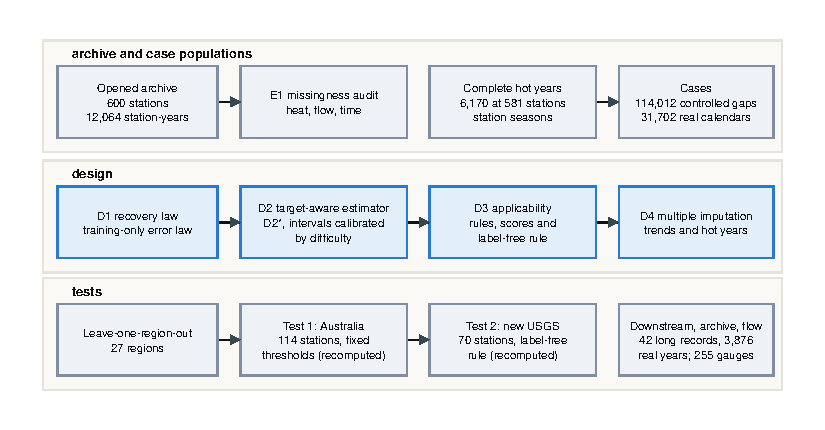
\includegraphics[width=\textwidth]{figures/tr_s1_design.pdf}
\caption{Study design. The archive and case populations feed four design components (D1--D4). They are tested by leave-one-region-out transfer, two preregistered tests on data not used in development (Australia with fixed thresholds; new USGS stations with the label-free rule), both recomputed after their first evaluation (Text~S6), a downstream trend experiment, an application to real incomplete years and a low-flow demonstration.}
\label{fig:design}
\end{figure}

\section{Archive, forcing, regions and hot years}
The archive combines daily water temperature from the U.S. Geological Survey, the Bavarian, Baden-W\"urttemberg, Czech, Slovenian, Swiss, Norwegian, Finnish and Dutch agencies, the French Hub'Eau service and the UK Environment Agency, assembled and quality-controlled for an earlier study. A station enters the case populations when it has at least four complete years. Air temperature is the NASA POWER daily 2-m temperature at the station coordinates. For 132 USGS stations added after the original forcing was built, the same product was retrieved from the coordinates in the USGS site service; 11 stations without coordinates have no air layer. Daily discharge (parameter 00060, statistic 00003) was retrieved from the USGS daily-value service; 287 of 336 USGS stations returned discharge. Independence groups join networks that share any station record. Regions are the European agencies and, for USGS stations, the two-digit hydrologic unit from the site service. Transfer analyses use the 14 regions with at least five independence groups.

\paragraph{Hot years and station seasons.} Records of stations south of the equator are shifted by 184 days before any year is formed, so that each analysis year runs from July to June; northern records are not shifted. For each case, the smoothed day-of-year climatology of the training years gives the station's five hottest consecutive months (its warm season, used by the warm-season features, the warm-season rules and the recovery-law moments) and its four hottest months (the degree-day target). The climatological peak window is the 30-day window with the highest training climatology; its centre anchors the peak-season rules (below). None of these quantities uses the target year. Table~S18 compares the corrected and the original definitions: in the source, masks, true H30, plug-in values and information layers are identical case by case, \TDefWarmNotMaySep{} of \TDefStations{} stations have a warm season other than May--September, \TDefDDNotJunSep{} have degree-day months other than June--September, and \TDefWarmChanged\% of the cases have a different warm-season observed fraction. In Australia the share of station-years whose H30 window touches the year boundary falls from \TAuEdgeBefore\% to \TAuEdgeAfter\%.

\section{Missingness audit}
The station-year sample contains fully operational years from 1982 onwards, excluding the first and last calendar year of each record, with summer (June--August) air temperature available. The summer anomaly is standardized within station. The conditional logit uses the station as stratum, so all between-station differences in maintenance and climate are removed; the mixed model adds random intercepts for station and for region $\times$ year, which absorbs regional shocks such as an agency-wide outage. For the daily analysis, a day is at risk when the station is active, the month is May--September and the previous day was observed; a gap onset is an at-risk day that is missing. Strata of station $\times$ year $\times$ month compare onset days with non-onset days of the same station-month, which controls for seasonality, station and year by design. The 7-day air anomaly is the departure from a 31-day smoothed day-of-year climatology averaged over the preceding week and standardized by its warm-season standard deviation at the station. Low flow means daily discharge below the 20th percentile of the station's record for that calendar month. Gap duration was regressed on the onset anomaly with station and month effects. Hot summers are the top 10\% of years by the region's mean standardized summer anomaly, for regions with at least ten years. The implied bias of a complete-years-only H30 climatology uses each station's regression of water H30 on air H30 in complete years and the difference in mean air H30 between complete years and all years. USGS daily values carry no cause code for missing days (all 68,180 missing days examined in an earlier audit), so gaps could not be split by cause. The audit uses Northern Hemisphere stations only and is unaffected by the corrected definitions. Table~S1 lists all models.

\section{Case populations, estimators, interval calibration and learning}
\paragraph{Masks.} The controlled population places one contiguous 30-, 60- or 90-day gap whose overlap with the training-period climatological 30-day peak window is zero, between 15\% and 85\%, or complete, twice per cell. The deployment population draws, without replacement, six real incomplete station-years of the same agency (fully operational years with at least one missing day) and moves each of their gaps by a uniform shift of up to 15 days (gaps touching the start or end of the year are not moved). Calendars leaving fewer than 30 observed days are skipped. The agency weights equal the agency's share of real incomplete station-years divided by its share of calendar cases. The state-dependent populations reweight calendar cases by the exact likelihood ratio between onset probabilities proportional to $\exp(k\beta z_t)$ and the uniform shift (main text); $\beta$ is the case-crossover log odds ratio of the 7-day air anomaly (\TOrOnset{} per standard deviation) and its upper 95\% bound gives a further stress level.

\paragraph{Plug-in and process estimators.} Neighbour regressions use the neighbours observed on at least 90\% of the hidden days and two annual harmonics; air regressions use air temperature at lags 0, 1, 2, 3, 5, 7 and 14 days and one harmonic; both are ridge regressions with unit penalty fitted on all non-target days. Air2stream-3 is calibrated by bounded least squares on the longest air-temperature segment outside the target year and integrated over each gap from the preceding observation.

\paragraph{Conditional simulation.} The residual history is the out-of-fold residual of the chosen reconstruction on each training year. Raw residual blocks resample 14-day blocks. The air-state law draws a slow 60-day residual path from a training year chosen with weights that compare its residuals on visible days and its air anomaly on the hidden days with those of the target year, and adds seasonally matched 14-day blocks of the fast residual. Each case has 128 draws.

\paragraph{Learning.} P2, P5a, P5b and the direct failure classifiers are LightGBM models (300 trees, learning rate 0.05, 31 leaves, at least 50 cases per leaf, 80\% row and column subsampling) on decision-time features only: gap geometry, the overlap with the climatological peak, the information layer, donor number and correlation, the recovery-law inputs, the air anomaly over the gap and the warm season, the visible water anomaly next to the gaps, the disagreement among reconstructions, out-of-fold reconstruction diagnostics, and the other reconstructions and the recorded-day value relative to the plug-in. P5b and the classifiers add the quantiles of both simulations relative to the plug-in. Every model is fitted 27 times, leaving out one region, and predicts only the held-out region. Quantile crossing is removed by sorting. For each of the two tests, the same models were refitted on all source cases and frozen.

\paragraph{Interval calibration.} For each quantile level $\tau$ of D2* and each decision-time group $g$ (share of the climatological peak window hidden: zero, or one of four quarters; information layer: neighbour, air, other, with groups below 300 cases merged into the air layer), the offset is the conformal quantile of the residuals $y - q_\tau$ of the calibration cases: the $\lceil (n+1)\tau \rceil$-th order statistic for $\tau \geq 0.5$ and the $\lfloor (n+1)\tau \rfloor$-th for $\tau < 0.5$ \cite{romano2019}. Offsets for a region are estimated on the other regions; the frozen models use offsets estimated on all source cases. Calibrated quantiles are sorted. Table~S19 gives the coverage and width of the 90\% interval in each group before and after calibration. The preset criterion (85--95\% in every group) was not met because the groups with a visible peak over-cover: a large share of their errors is exactly zero, and no quantile of a distribution with a point mass can be placed to cover exactly 90\%. The intervals are therefore reported as approximate, with coverage by group.

\section{Recovery law, rules and tolerance sensitivity}
\paragraph{Derivation.} Let $p_t$ be the reconstruction and $a_t = y_t - s_t$ the anomaly. For a conditional-mean reconstruction, $r_t = p_t - y_t$ is uncorrelated with $p_s$, so $\mathrm{Cov}(r_t, a_s) = -\mathrm{Cov}(r_t, r_s) = -\sigma_r^2\phi_r^{|t-s|}$ for an AR(1) residual. The hottest window $\mathcal S$ is selected on $\bar a_{\mathcal S}$, whose variance is $\sigma_a^2 v(30,\phi_a)$. Linear prediction of the hidden residual mean from $\bar a_{\mathcal S}$ gives the slope $\kappa_m$ of the main text, and the conditional variance follows from the same covariances. The daily-scale version (v1) replaces $\kappa_m$ by $1-R^2 = \sigma_r^2/\sigma_a^2$ and the conditional variance by $\sigma_r^2 R^2 v(m,\phi_r)$; it overstates the shrinkage whenever the residual is less persistent than the anomaly. The peak-window version (v2p) takes the mean and standard deviation of the out-of-fold residuals inside the training years' peak windows instead of the warm-season moments and the shrinkage term. The replay (v3) applies the current mask to each training year, completes the hidden days with that year's out-of-fold residuals and takes the empirical distribution of the resulting H30 errors, smoothed with a Gaussian kernel; it is an empirical comparator, not a law. Tables~S3 and S4 compare the versions at case and cell level.

\paragraph{Hard cells.} In the five cells with the highest observed failure rate among cells with at least 200 cases, the law predicted \THardVTwo\% against \THardObserved\% observed (v2p: \THardVTwoP\%). The standardized errors $(e-\hat\mu)/\hat\sigma$ exceeded two in absolute value in \THardBeyond\% of these cases, the excess kurtosis of the errors was \THardKurtosis{} and their variance was \THardVariance\% larger than the law's. The ratio of the residual standard deviation inside the peak windows to its warm-season value was \THardHetero, so the shortfall comes from heavy tails rather than from larger residuals in hot periods.

\paragraph{Rules.} Rules are applied to the case's missing-day mask in its hot year. The USGS indicator rule requires at least 311 observed days and at least 24 per month; its strict form requires 26 per month and no 7-day window with more than one missing day. The WMO 11/5 rule requires every month to have fewer than 11 missing days and no run of five or more. ETCCDI requires at most 15 missing days in the year and at most three per month; GSIM at least 350 observed days. The peak-season rules evaluate July--September, August, July--August and 15 July--15 September as written for Northern Hemisphere streams whose peak is near 30 July (day 211). We move these windows by the difference between the station's climatological peak centre and day 211, which keeps their position relative to the peak; Table~2 of the main text also reports them as written. The NRFA-type rule scores a year by the position of its best fully observed 30-day mean in the training distribution of H30. Table~2 of the main text adds, for each fixed rule, the failure rate of the plug-in among the rejected years and, for rules with a free threshold, the result when the threshold is chosen on the other regions.

\paragraph{Tolerance and risk.} Table~S16 repeats the main comparison at 0.25 and 1.0\,$^{\circ}$C. Retention at 2.5\% and 10\% risk is in Table~S7.

\section{Transfer, the two preregistered tests and post hoc diagnosis}
\paragraph{Fixed thresholds (first preregistration).} A threshold is the largest score at which the weighted failure rate of all calibration cases with a lower score is at most 5\%. Mondrian calibration does this within the neighbour layer, the air layer and the remaining layers. Covariate-shift weights are the odds of a classifier that separates the held-out region's cases from the calibration cases on decision-time features. Local recalibration draws $k$ independence groups from the held-out region, either alone or added to the source with up-weighting, and evaluates the remaining groups; it is repeated 30 times. The random-effects model treats the logit of each region's realised risk as normal with a region-level variance and uses an effective sample size capped at 30 cases per independence group. Table~S9 gives the regional results.

\paragraph{First test.} The Australian roster, coordinates, network assignment and air forcing were prepared without computing any water-temperature statistic beyond completeness counts. The models, thresholds, estimator selection, preregistration and all code used by the evaluation were frozen before it first ran. Table~S10 reports the outcome of the recomputation (Text~S6). Written after this evaluation, the post hoc analyses compare recoverability parameters, gap calendars, failure rates and score calibration between the source and Australia (Tables~S11 and S17).

\paragraph{Label-free rule.} For a set of cases with predicted failure probabilities $\hat p_i$ sorted in increasing order, the rule admits the largest prefix whose mean of $k\hat p_i$ is at most 5\%; tied scores are admitted together. In development, the rule was applied separately in each held-out region and population. The factor for a held-out region is the 80th percentile, over the other regions, of the ratio between realised and mean predicted risk among the cases admitted with $k=1$, and at least one; the frozen factor uses all regions. Table~S12 lists every region and the post hoc results in Australia under the corrected definitions, where the candidate models that were later frozen were applied to the opened Australian cases.

\paragraph{Second test.} The candidates were the \TNewCandidates{} USGS stations that an earlier metadata intake had retained because no record of them had been cached or analysed and no known network connection linked them to analysed stations. For each, only the dates of approved daily means and their approval status were requested from the USGS daily collection, with the request fields restricted to time and approval status. Complete years (every day approved), the active span, the share of incomplete active years and their gap calendars were derived from these dates. Eligible targets have at least four complete years (\TNewStationsDesign{} stations); every candidate in the same eight-digit hydrologic unit as a target is a member of its network and a potential donor. Independence groups join stations that share a hydrologic unit or an intake network component. The missingness stratum is high when at least half of the active years are incomplete. NASA POWER air temperature was retrieved for the targets with the same request as for the source. The second preregistration was written and a copy was saved, and the configuration, the models, the conformal offsets, the rule and its factor, the design roster, the air forcing, the two versions of the results section and all code were frozen; only then were the approved daily values of all members requested, quality-controlled with the repository's ingest checks and arranged by network. Calendar cases of a target draw from its own incomplete years, then from its network's, then from all new stations. Table~S20 gives the results of the recomputation (Text~S6). The local calibration analysis draws $m = 2, 4, 8, 16$ labelled groups, re-estimates $k$ from them as above, applies the rule to the remaining groups, and repeats 500 times.

\section{Preregistrations, freeze and deviations}
\paragraph{First preregistration.} It was written after the missingness audit and before any estimator comparison. It fixed the populations, independent units, primary target and tolerances, four primary endpoints with success criteria, Holm control, the decision gates and the test region. The machine-readable file was written at 21:00:09 UTC on 21 October 2026 and the document at 21:00:56; the first full case table was written at 21:04:29 and the first failure rate of the deployment population was computed at 21:05:17. Before the preregistration, a one-station case table (240 cases) was inspected once to check the code; its mean signed errors by design type were printed, but no failure rate. The document was changed once, at 21:23:45 and before the downstream experiment, by appending the clarification of P4 below. Its as-written version is archived.

\paragraph{Second preregistration.} It was written after the source development of the corrected definitions, the interval calibration and the label-free rule, after the Australian development check, and after the availability-only design of the second test; no water-temperature value of the new stations had been requested. A copy was saved at the moment of writing, and the pipeline was frozen seconds later (07:39:19 and 07:39:22 UTC on 22 October 2026).

\paragraph{Deviations.}
\begin{enumerate}
\item Before the downstream experiment ran, the coverage criterion of P4 was clarified to refer to the missing-data component of the multiple-imputation interval around the complete-record slope.
\item P3 requires success in both populations, the stricter reading of ``mech + deploy''.
\item The recovery law gained the window-scale version (v2) and the replay (v3) during development; v1 is reported. All three were fixed before the first freeze; v2p was added in the revision.
\item A first run of the downstream experiment used large-sample Rubin degrees of freedom; the reported results use Barnard--Rubin degrees of freedom.
\item The label-free threshold was formulated after the first test; it was developed on the source and evaluated in the second test under the second preregistration. Australian results under this rule are post hoc.
\item Return levels, a cause-specific missingness analysis and a natural-gap comparison with independent reference sensors were not possible with the available data.
\item The first frozen pipeline used calendar years and a May--September warm season, which is not adapted to the Southern Hemisphere. In the revision, all analyses use hot years and station seasons; the verdicts of P1--P4 are those of the registered analysis, and the corrected values are reported beside them.
\item After the first preregistration and before the first freeze, the case builder gained outputs for the ablations (unshrunk air regression, the earlier peak-window summaries, training-year replay errors) and a mode for real incomplete years. All previously existing columns were verified to be identical after the rebuild. The ``case table at the time of preregistration'' in the first version of this deviation is the first full table, completed five minutes after the preregistration.
\item Gate C anticipated a short note if P2 failed. P2 failed because D2* without screening already met the 5\% risk under real calendars, which makes the gain at 5\% uninformative rather than negative; the main claims rest on P1, P4 and the screening of long gaps, so the study is reported as a full article.
\item The interval calibration by difficulty group was added after P1 had been evaluated; P1 is judged on the registered uncalibrated intervals.
\item The peak-season rules are anchored to each station's climatological peak in the revision; the rules as written are reported in Table~2 of the main text.
\item The low-flow demonstration and the decomposition of the downstream gain were added in the revision and are exploratory.
\item After both tests had been evaluated, the generation of random numbers was changed so that every seed is a plain integer (a fixed number, or one formed from the position of a station or region in a sorted list, the year and the step of the design). This redrew every mask, calendar draw, shift, simulation and resample. All results were recomputed with otherwise unchanged definitions, models, rules and code; the machine-readable preregistration files were regenerated by the same code, with a new creation time. The original evaluations, which can no longer be reproduced exactly, gave: P1 a reduction of 73\% with 85.1\% coverage (met); P2 a gain of 0.0 points (not met); P3 86\% of regions under long gaps (median 5.7\%), 93\% under real calendars, and 12.6\% and 17.5\% realised risk in Australia (not met); P4 a reduction of 76\% with 95.9\% coverage (met); N1 4.4\% (upper bound 6.2\%) under real calendars and 5.1\% (6.3\%) under long gaps with $k=1.27$ (met); N2 87.9\% coverage (met); N3 a reduction of 88\% (met); N4 gains of 44 and 2 points. In the recomputation P1 is not met, because its coverage of 84.8\% fell just below the registered floor of 85\%, and P3 is not met with 79\% of regions under long gaps (median 5.6\%) and Australian risks of 13.1\% and 17.6\%; P4 is met with a reduction of 65\% (67\% under the corrected definitions); N1--N3 are met (4.5\% and 5.6\% realised risk with $k=1.27$, 87.4\% coverage, a bias reduction of 86\%), and local re-estimation of $k$ needed eight labelled groups under long gaps instead of two. The main text and the tables report the recomputed values. Because the change was made after both outcomes were known, neither test is reported as blind.
\end{enumerate}

\section{Downstream decomposition and the 7-day minimum flow}
\paragraph{Decomposition.} For each station and pipeline, the trend RMSE is computed over the 200 degradations. The share of the A1-to-C reduction obtained by keeping years is $(\mathrm{RMSE}_{A1}-\mathrm{RMSE}_{B})/(\mathrm{RMSE}_{A1}-\mathrm{RMSE}_{C})$ over all stations, with an interval from resampling independence groups. Station ratios are undefined where the denominator pipeline is exact; at \TNStationsBExact{} stations no transplanted calendar reached the peak window and the plug-in was exact. Detection of warming uses the $t$ interval of each pipeline (Barnard--Rubin degrees of freedom for C). The Baden-W\"urttemberg trends use the 19 stations with at least five complete years and at least 15 years in total, and the same 20 multiple imputations per incomplete year as in the main analysis; the anomaly series are the year effects of a least-squares model with station and year effects, centred on zero (Table~S21).

\paragraph{Low flow.} Discharge values with an approval code (including approved estimates) are valid; streams with any zero flow are excluded because the log error of 7Q is undefined when 7Q is zero. A climatic year runs from 1 April to 31 March and is complete when every day is valid. The climatology of log flow is a 31-day circular moving average of the training years' day-of-year means, and the low-flow window is the 30 days centred on the median position of the training years' 7Q. Controlled gaps of 30, 60 and 90 days have no, partial or full overlap with this window (one per cell); real calendars come from the 155 interior incomplete climatic years with at least 30 valid days, moved by up to 15 days, six per complete year. Neighbours lie within 200\,km, have an anomaly correlation of at least 0.6 over at least three years of common training days and are complete in the target year; at most three are used in a ridge regression with unit penalty. The target-aware estimator predicts seven quantiles of the log error with the same LightGBM settings as P5a, from the missing fraction, the number and longest length of gaps, the overlap with the low-flow window, gaps at the year boundary, the layer, the number of neighbours and the regression $R^2$, the plug-in 7Q relative to the training mean, the recorded-day 7Q relative to the plug-in, the best neighbour's 7Q anomaly in the target year, the training standard deviation of log 7Q, the distance of the gap centre from the low-flow window and the visible anomaly next to the gaps. The trend experiment degrades each station with at least 20 complete climatic years 200 times at random, with the station's real share of incomplete years (between 5\% and 60\%), and estimates the OLS trend of log 7Q per decade. Table~S22 gives the results.

\clearpage
\begin{table}
\caption{E1 missingness models. Station-year models use station fixed effects (conditional logit) or station and region-year random intercepts; onset models are time-stratified case-crossover designs (strata: station $\times$ year $\times$ month). Duration is a ratio of gap lengths. Intervals resample independence groups (model-based for the mixed model and duration).}
\label{tab:si_e1}
\centering
\scriptsize
\fittable{%
\begin{tabular}{llrl}
\toprule
Analysis & Covariate & n & Odds ratio [95\%] \\
\midrule
station year conditional logit & z air & 8{,}848 & 1.06 [1.00, 1.13] \\
station year conditional logit & trend & 8{,}848 & 0.68 [0.59, 0.81] \\
station year conditional logit below90 & z air & 6{,}275 & 1.03 [0.95, 1.11] \\
station year conditional logit below90 & trend & 6{,}275 & 0.62 [0.50, 0.76] \\
station year conditional logit julaug & z air & 8{,}148 & 1.06 [0.99, 1.13] \\
station year conditional logit julaug & trend & 8{,}148 & 0.68 [0.59, 0.80] \\
station year conditional logit usgs flow & z air & 4{,}632 & 1.02 [0.94, 1.12] \\
station year conditional logit usgs flow & z flow & 4{,}632 & 0.94 [0.87, 1.01] \\
station year conditional logit usgs flow & trend & 4{,}632 & 0.66 [0.54, 0.81] \\
station year mixed station region year & z air & 10{,}580 & 1.13 [1.07, 1.18] \\
station year mixed station region year & trend & 10{,}580 & 0.59 [0.57, 0.61] \\
onset case crossover air & z air week & 105{,}238 & 1.07 [1.01, 1.12] \\
onset case crossover air water & z air week & 105{,}238 & 1.07 [1.02, 1.11] \\
onset case crossover air water & z water lag & 105{,}238 & 1.01 [0.96, 1.07] \\
onset case crossover usgs flow & z air week & 61{,}052 & 1.06 [0.99, 1.12] \\
onset case crossover usgs flow & low flow & 61{,}052 & 1.17 [0.93, 1.55] \\
gap log duration station fe & z air week & 5{,}392 & 0.98 [0.94, 1.01] \\
\bottomrule
\end{tabular}
}
\end{table}

\begin{table}
\caption{Target tolerances: the share of the median within-station interannual standard deviation that 0.5\,$^{\circ}$C represents for H30, with floors of 0.2\,$^{\circ}$C and one day, recomputed for the degree-days of each station's four climatologically hottest months.}
\label{tab:si_tolerance}
\centering
\scriptsize
\fittable{%
\begin{tabular}{lrr}
\toprule
Target & Median interannual SD & Tolerance \\
\midrule
Annual mean & 0.53 & 0.26 \\
C30 & 0.80 & 0.40 \\
Days $>$20\,$^{\circ}$C & 10.95 & 5.45 \\
Degree-days, 4 hottest months & 94.36 & 46.97 \\
H30 & 1.00 & 0.50 \\
H7 & 1.07 & 0.53 \\
\bottomrule
\end{tabular}
}
\end{table}

\begin{table}
\caption{E3 recovery law, case level. v1: daily-scale shrinkage; v2: window-scale shrinkage (main parametric law); v2p: residual moments inside the training peak windows; v3: replay of the same gap on training years (empirical comparator). No version is fitted to reconstruction errors.}
\label{tab:si_law}
\centering
\scriptsize
\fittable{%
\begin{tabular}{llrrrrrrr}
\toprule
Population & Law & ECE & Brier skill & AUC & Predicted failure & Observed failure & Predicted bias & Observed bias \\
\midrule
deploy & v1 & 0.002 & 0.426 & 0.978 & 0.032 & 0.033 & \ensuremath{-}0.038 & \ensuremath{-}0.026 \\
deploy & v2 & 0.002 & 0.428 & 0.978 & 0.032 & 0.033 & \ensuremath{-}0.036 & \ensuremath{-}0.026 \\
deploy & v2p & 0.006 & 0.418 & 0.979 & 0.037 & 0.033 & \ensuremath{-}0.051 & \ensuremath{-}0.026 \\
deploy & v3 & 0.009 & 0.412 & 0.978 & 0.037 & 0.032 & \ensuremath{-}0.027 & \ensuremath{-}0.026 \\
mech & v1 & 0.023 & 0.266 & 0.866 & 0.148 & 0.170 & \ensuremath{-}0.147 & \ensuremath{-}0.064 \\
mech & v2 & 0.027 & 0.266 & 0.867 & 0.143 & 0.170 & \ensuremath{-}0.133 & \ensuremath{-}0.064 \\
mech & v2p & 0.027 & 0.274 & 0.869 & 0.165 & 0.170 & \ensuremath{-}0.187 & \ensuremath{-}0.064 \\
mech & v3 & 0.039 & 0.256 & 0.863 & 0.182 & 0.171 & \ensuremath{-}0.063 & \ensuremath{-}0.068 \\
\bottomrule
\end{tabular}
}
\end{table}

\begin{table}
\caption{E3 cells of the controlled population (gap length $\times$ overlap with the climatological peak $\times$ information layer).}
\label{tab:si_cells}
\centering
\tiny
\fittable{%
\begin{tabular}{rllrrrrrrrr}
\toprule
Days & Overlap & Layer & n & Mean error & v2 bias & v3 bias & Failure & v2 P(fail) & v2p P(fail) & v3 P(fail) \\
\midrule
30 & full & air ridge & 1{,}964 & \ensuremath{-}0.290 & \ensuremath{-}0.331 & \ensuremath{-}0.293 & 0.401 & 0.341 & 0.428 & 0.432 \\
30 & full & donor ridge & 10{,}422 & \ensuremath{-}0.002 & \ensuremath{-}0.134 & \ensuremath{-}0.020 & 0.185 & 0.152 & 0.175 & 0.210 \\
30 & none & air ridge & 1{,}742 & \ensuremath{-}0.002 & \ensuremath{-}0.014 & \ensuremath{-}0.003 & 0.013 & 0.009 & 0.011 & 0.010 \\
30 & none & donor ridge & 10{,}670 & 0.001 & \ensuremath{-}0.009 & 0.002 & 0.006 & 0.004 & 0.005 & 0.006 \\
30 & partial & air ridge & 1{,}909 & \ensuremath{-}0.185 & \ensuremath{-}0.259 & \ensuremath{-}0.153 & 0.260 & 0.237 & 0.307 & 0.295 \\
30 & partial & donor ridge & 10{,}495 & \ensuremath{-}0.006 & \ensuremath{-}0.119 & \ensuremath{-}0.004 & 0.132 & 0.104 & 0.121 & 0.143 \\
60 & full & air ridge & 3{,}119 & \ensuremath{-}0.440 & \ensuremath{-}0.386 & \ensuremath{-}0.417 & 0.519 & 0.459 & 0.528 & 0.537 \\
60 & full & donor ridge & 9{,}319 & \ensuremath{-}0.055 & \ensuremath{-}0.167 & \ensuremath{-}0.056 & 0.281 & 0.229 & 0.254 & 0.302 \\
60 & full & smooth climatology & 114 & \ensuremath{-}0.435 & \ensuremath{-}0.766 & \ensuremath{-}0.399 & 0.658 & 0.672 & 0.717 & 0.674 \\
60 & none & air ridge & 2{,}679 & \ensuremath{-}0.011 & \ensuremath{-}0.025 & \ensuremath{-}0.002 & 0.018 & 0.015 & 0.018 & 0.016 \\
60 & none & donor ridge & 9{,}760 & 0.001 & \ensuremath{-}0.012 & 0.001 & 0.008 & 0.006 & 0.007 & 0.007 \\
60 & none & smooth climatology & 117 & \ensuremath{-}0.016 & \ensuremath{-}0.032 & \ensuremath{-}0.014 & 0.009 & 0.019 & 0.022 & 0.012 \\
60 & partial & air ridge & 2{,}979 & \ensuremath{-}0.208 & \ensuremath{-}0.286 & \ensuremath{-}0.180 & 0.286 & 0.261 & 0.328 & 0.313 \\
60 & partial & donor ridge & 9{,}451 & \ensuremath{-}0.011 & \ensuremath{-}0.137 & \ensuremath{-}0.011 & 0.153 & 0.124 & 0.143 & 0.167 \\
60 & partial & smooth climatology & 118 & \ensuremath{-}0.163 & \ensuremath{-}0.538 & \ensuremath{-}0.207 & 0.364 & 0.403 & 0.476 & 0.460 \\
90 & full & air ridge & 3{,}869 & \ensuremath{-}0.500 & \ensuremath{-}0.402 & \ensuremath{-}0.470 & 0.552 & 0.499 & 0.565 & 0.570 \\
90 & full & donor ridge & 8{,}596 & \ensuremath{-}0.073 & \ensuremath{-}0.176 & \ensuremath{-}0.074 & 0.312 & 0.256 & 0.282 & 0.335 \\
90 & full & smooth climatology & 118 & \ensuremath{-}0.534 & \ensuremath{-}0.850 & \ensuremath{-}0.464 & 0.695 & 0.708 & 0.742 & 0.700 \\
90 & none & air ridge & 3{,}523 & \ensuremath{-}0.014 & \ensuremath{-}0.032 & \ensuremath{-}0.008 & 0.023 & 0.020 & 0.023 & 0.020 \\
90 & none & donor ridge & 8{,}937 & 0.001 & \ensuremath{-}0.017 & 0.002 & 0.011 & 0.008 & 0.009 & 0.011 \\
90 & none & smooth climatology & 122 & \ensuremath{-}0.027 & \ensuremath{-}0.031 & \ensuremath{-}0.015 & 0.025 & 0.019 & 0.021 & 0.011 \\
90 & partial & air ridge & 3{,}746 & \ensuremath{-}0.204 & \ensuremath{-}0.288 & \ensuremath{-}0.179 & 0.294 & 0.260 & 0.326 & 0.307 \\
90 & partial & donor ridge & 8{,}703 & \ensuremath{-}0.011 & \ensuremath{-}0.144 & \ensuremath{-}0.015 & 0.161 & 0.128 & 0.148 & 0.171 \\
90 & partial & smooth climatology & 121 & \ensuremath{-}0.203 & \ensuremath{-}0.499 & \ensuremath{-}0.185 & 0.421 & 0.372 & 0.453 & 0.428 \\
\bottomrule
\end{tabular}
}
\end{table}

\begin{table}
\caption{E4 H30 estimators, leave-one-region-out, before interval calibration. Strata use the true peak window (evaluation only); warm anomaly: true H30 at least 1\,$^{\circ}$C above the training mean. Calibrated coverage by difficulty group is in Table~\ref{tab:si_conformal}.}
\label{tab:si_estimators}
\centering
\tiny
\fittable{%
\begin{tabular}{lllrrrrrr}
\toprule
Population & Stratum & Estimator & n & Bias & MAE & Failure (\%) & CRPS & Cover90 (\%) \\
\midrule
mech & all & P0 plug-in & 112{,}593 & \ensuremath{-}0.064 & 0.260 & 17.0 & -- & -- \\
mech & all & Recorded days only & 112{,}593 & \ensuremath{-}0.781 & 0.802 & 38.7 & -- & -- \\
mech & all & Air2stream-3 & 110{,}609 & \ensuremath{-}0.090 & 0.325 & 23.4 & -- & -- \\
mech & all & P2 functional debiasing & 112{,}593 & 0.004 & 0.209 & 12.7 & -- & -- \\
mech & all & P3 air-state simulation & 112{,}593 & \ensuremath{-}0.011 & 0.223 & 14.3 & 0.134 & 88.3 \\
mech & all & P3 raw residual blocks & 112{,}593 & \ensuremath{-}0.024 & 0.254 & 16.7 & 0.162 & 81.1 \\
mech & all & P5a distribution regression & 112{,}593 & \ensuremath{-}0.019 & 0.203 & 12.6 & 0.122 & 90.0 \\
mech & all & P5b = D2* & 112{,}593 & \ensuremath{-}0.016 & 0.197 & 12.0 & 0.118 & 90.2 \\
mech & peak half hidden & P0 plug-in & 49{,}935 & \ensuremath{-}0.174 & 0.493 & 33.9 & -- & -- \\
mech & peak half hidden & Recorded days only & 49{,}935 & \ensuremath{-}1.712 & 1.714 & 82.1 & -- & -- \\
mech & peak half hidden & Air2stream-3 & 49{,}072 & \ensuremath{-}0.230 & 0.626 & 47.0 & -- & -- \\
mech & peak half hidden & P2 functional debiasing & 49{,}935 & \ensuremath{-}0.059 & 0.375 & 24.9 & -- & -- \\
mech & peak half hidden & P3 air-state simulation & 49{,}935 & \ensuremath{-}0.060 & 0.417 & 28.2 & 0.249 & 81.2 \\
mech & peak half hidden & P3 raw residual blocks & 49{,}935 & \ensuremath{-}0.096 & 0.473 & 32.9 & 0.301 & 68.4 \\
mech & peak half hidden & P5a distribution regression & 49{,}935 & \ensuremath{-}0.089 & 0.380 & 25.4 & 0.227 & 83.3 \\
mech & peak half hidden & P5b = D2* & 49{,}935 & \ensuremath{-}0.080 & 0.370 & 24.2 & 0.220 & 84.0 \\
mech & air layer half hidden & P0 plug-in & 12{,}325 & \ensuremath{-}0.473 & 0.732 & 52.4 & -- & -- \\
mech & air layer half hidden & Recorded days only & 12{,}325 & \ensuremath{-}1.861 & 1.863 & 84.6 & -- & -- \\
mech & air layer half hidden & Air2stream-3 & 12{,}325 & \ensuremath{-}0.250 & 0.634 & 46.9 & -- & -- \\
mech & air layer half hidden & P2 functional debiasing & 12{,}325 & \ensuremath{-}0.096 & 0.460 & 33.1 & -- & -- \\
mech & air layer half hidden & P3 air-state simulation & 12{,}325 & \ensuremath{-}0.171 & 0.510 & 37.0 & 0.304 & 82.8 \\
mech & air layer half hidden & P3 raw residual blocks & 12{,}325 & \ensuremath{-}0.329 & 0.657 & 48.8 & 0.407 & 70.1 \\
mech & air layer half hidden & P5a distribution regression & 12{,}325 & \ensuremath{-}0.144 & 0.473 & 34.2 & 0.281 & 84.3 \\
mech & air layer half hidden & P5b = D2* & 12{,}325 & \ensuremath{-}0.137 & 0.458 & 32.3 & 0.272 & 84.8 \\
mech & donor layer half hidden & P0 plug-in & 37{,}271 & \ensuremath{-}0.072 & 0.410 & 27.5 & -- & -- \\
mech & donor layer half hidden & Recorded days only & 37{,}271 & \ensuremath{-}1.654 & 1.657 & 81.3 & -- & -- \\
mech & donor layer half hidden & Air2stream-3 & 36{,}747 & \ensuremath{-}0.223 & 0.623 & 47.1 & -- & -- \\
mech & donor layer half hidden & P2 functional debiasing & 37{,}271 & \ensuremath{-}0.046 & 0.343 & 21.8 & -- & -- \\
mech & donor layer half hidden & P3 air-state simulation & 37{,}271 & \ensuremath{-}0.022 & 0.382 & 25.0 & 0.228 & 80.7 \\
mech & donor layer half hidden & P3 raw residual blocks & 37{,}271 & \ensuremath{-}0.017 & 0.408 & 27.3 & 0.264 & 67.8 \\
mech & donor layer half hidden & P5a distribution regression & 37{,}271 & \ensuremath{-}0.069 & 0.345 & 22.2 & 0.206 & 83.0 \\
mech & donor layer half hidden & P5b = D2* & 37{,}271 & \ensuremath{-}0.060 & 0.337 & 21.2 & 0.200 & 83.8 \\
mech & warm anomaly half hidden & P0 plug-in & 9{,}995 & \ensuremath{-}0.623 & 0.727 & 50.1 & -- & -- \\
mech & warm anomaly half hidden & Recorded days only & 9{,}995 & \ensuremath{-}2.262 & 2.265 & 90.9 & -- & -- \\
mech & warm anomaly half hidden & Air2stream-3 & 9{,}833 & \ensuremath{-}0.717 & 0.893 & 64.8 & -- & -- \\
mech & warm anomaly half hidden & P2 functional debiasing & 9{,}995 & \ensuremath{-}0.387 & 0.513 & 36.7 & -- & -- \\
mech & warm anomaly half hidden & P3 air-state simulation & 9{,}995 & \ensuremath{-}0.472 & 0.603 & 43.8 & 0.365 & 67.3 \\
mech & warm anomaly half hidden & P3 raw residual blocks & 9{,}995 & \ensuremath{-}0.566 & 0.681 & 48.8 & 0.463 & 51.1 \\
mech & warm anomaly half hidden & P5a distribution regression & 9{,}995 & \ensuremath{-}0.424 & 0.538 & 38.5 & 0.328 & 73.1 \\
mech & warm anomaly half hidden & P5b = D2* & 9{,}995 & \ensuremath{-}0.402 & 0.524 & 37.4 & 0.318 & 73.4 \\
deploy & all & P0 plug-in & 31{,}178 & \ensuremath{-}0.026 & 0.060 & 3.3 & -- & -- \\
deploy & all & Recorded days only & 31{,}114 & \ensuremath{-}0.313 & 0.330 & 7.0 & -- & -- \\
deploy & all & Air2stream-3 & 26{,}176 & \ensuremath{-}0.013 & 0.041 & 2.2 & -- & -- \\
deploy & all & P2 functional debiasing & 31{,}178 & 0.000 & 0.051 & 2.7 & -- & -- \\
deploy & all & P3 air-state simulation & 31{,}178 & \ensuremath{-}0.007 & 0.050 & 2.8 & 0.029 & 94.9 \\
deploy & all & P3 raw residual blocks & 31{,}178 & \ensuremath{-}0.013 & 0.057 & 3.0 & 0.035 & 93.7 \\
deploy & all & P5a distribution regression & 31{,}178 & \ensuremath{-}0.002 & 0.045 & 2.5 & 0.027 & 97.2 \\
deploy & all & P5b = D2* & 31{,}178 & \ensuremath{-}0.003 & 0.044 & 2.4 & 0.026 & 97.3 \\
deploy & peak half hidden & P0 plug-in & 2{,}592 & \ensuremath{-}0.314 & 0.627 & 42.4 & -- & -- \\
deploy & peak half hidden & Recorded days only & 2{,}538 & \ensuremath{-}4.546 & 4.547 & 89.2 & -- & -- \\
deploy & peak half hidden & Air2stream-3 & 1{,}509 & \ensuremath{-}0.217 & 0.612 & 46.5 & -- & -- \\
deploy & peak half hidden & P2 functional debiasing & 2{,}592 & \ensuremath{-}0.040 & 0.483 & 34.5 & -- & -- \\
deploy & peak half hidden & P3 air-state simulation & 2{,}592 & \ensuremath{-}0.080 & 0.496 & 37.5 & 0.292 & 81.7 \\
deploy & peak half hidden & P3 raw residual blocks & 2{,}592 & \ensuremath{-}0.150 & 0.576 & 39.3 & 0.364 & 68.3 \\
deploy & peak half hidden & P5a distribution regression & 2{,}592 & \ensuremath{-}0.059 & 0.482 & 34.4 & 0.285 & 85.0 \\
deploy & peak half hidden & P5b = D2* & 2{,}592 & \ensuremath{-}0.064 & 0.470 & 33.5 & 0.274 & 85.5 \\
deploy & air layer half hidden & P0 plug-in & 828 & \ensuremath{-}0.489 & 0.778 & 53.3 & -- & -- \\
deploy & air layer half hidden & Recorded days only & 812 & \ensuremath{-}5.375 & 5.376 & 92.5 & -- & -- \\
deploy & air layer half hidden & Air2stream-3 & 424 & \ensuremath{-}0.177 & 0.646 & 49.5 & -- & -- \\
deploy & air layer half hidden & P2 functional debiasing & 828 & \ensuremath{-}0.051 & 0.533 & 39.0 & -- & -- \\
deploy & air layer half hidden & P3 air-state simulation & 828 & \ensuremath{-}0.122 & 0.544 & 42.9 & 0.320 & 82.2 \\
deploy & air layer half hidden & P3 raw residual blocks & 828 & \ensuremath{-}0.260 & 0.686 & 47.2 & 0.430 & 69.0 \\
deploy & air layer half hidden & P5a distribution regression & 828 & \ensuremath{-}0.079 & 0.541 & 39.5 & 0.319 & 86.4 \\
deploy & air layer half hidden & P5b = D2* & 828 & \ensuremath{-}0.091 & 0.522 & 38.7 & 0.304 & 86.0 \\
deploy & donor layer half hidden & P0 plug-in & 1{,}712 & \ensuremath{-}0.113 & 0.446 & 28.7 & -- & -- \\
deploy & donor layer half hidden & Recorded days only & 1{,}674 & \ensuremath{-}3.597 & 3.597 & 85.2 & -- & -- \\
deploy & donor layer half hidden & Air2stream-3 & 1{,}083 & \ensuremath{-}0.254 & 0.582 & 43.7 & -- & -- \\
deploy & donor layer half hidden & P2 functional debiasing & 1{,}712 & \ensuremath{-}0.034 & 0.414 & 27.9 & -- & -- \\
deploy & donor layer half hidden & P3 air-state simulation & 1{,}712 & \ensuremath{-}0.035 & 0.426 & 29.9 & 0.252 & 80.9 \\
deploy & donor layer half hidden & P3 raw residual blocks & 1{,}712 & \ensuremath{-}0.033 & 0.439 & 29.2 & 0.283 & 67.3 \\
deploy & donor layer half hidden & P5a distribution regression & 1{,}712 & \ensuremath{-}0.038 & 0.404 & 27.3 & 0.241 & 83.9 \\
deploy & donor layer half hidden & P5b = D2* & 1{,}712 & \ensuremath{-}0.038 & 0.399 & 26.4 & 0.234 & 84.9 \\
deploy & warm anomaly half hidden & P0 plug-in & 530 & \ensuremath{-}1.039 & 1.062 & 63.8 & -- & -- \\
deploy & warm anomaly half hidden & Recorded days only & 519 & \ensuremath{-}5.040 & 5.040 & 95.4 & -- & -- \\
deploy & warm anomaly half hidden & Air2stream-3 & 317 & \ensuremath{-}0.767 & 0.895 & 61.1 & -- & -- \\
deploy & warm anomaly half hidden & P2 functional debiasing & 530 & \ensuremath{-}0.672 & 0.727 & 54.7 & -- & -- \\
deploy & warm anomaly half hidden & P3 air-state simulation & 530 & \ensuremath{-}0.773 & 0.813 & 58.8 & 0.488 & 62.6 \\
deploy & warm anomaly half hidden & P3 raw residual blocks & 530 & \ensuremath{-}0.911 & 0.941 & 60.5 & 0.648 & 44.6 \\
deploy & warm anomaly half hidden & P5a distribution regression & 530 & \ensuremath{-}0.709 & 0.754 & 54.2 & 0.457 & 68.5 \\
deploy & warm anomaly half hidden & P5b = D2* & 530 & \ensuremath{-}0.698 & 0.751 & 53.5 & 0.446 & 68.4 \\
\bottomrule
\end{tabular}
}
\end{table}

\begin{table}
\caption{E4 estimators for the other targets (all cases), with the target tolerances.}
\label{tab:si_other_targets}
\centering
\tiny
\fittable{%
\begin{tabular}{lllrrr}
\toprule
Population & Target & Estimator & Bias & MAE & Failure (\%) \\
\midrule
mech & H7 & P0 plug-in & \ensuremath{-}0.100 & 0.284 & 18.0 \\
mech & H7 & Recorded days only & \ensuremath{-}0.647 & 0.651 & 31.7 \\
mech & H7 & P2 functional debiasing & 0.013 & 0.247 & 14.7 \\
mech & H7 & P3 air-state simulation & 0.001 & 0.252 & 16.6 \\
mech & H7 & P5b = D2* & \ensuremath{-}0.033 & 0.228 & 14.4 \\
mech & Annual mean & P0 plug-in & \ensuremath{-}0.003 & 0.076 & 4.8 \\
mech & Annual mean & Recorded days only & \ensuremath{-}0.836 & 1.134 & 90.3 \\
mech & Annual mean & P2 functional debiasing & 0.001 & 0.062 & 2.5 \\
mech & Annual mean & P3 air-state simulation & \ensuremath{-}0.000 & 0.067 & 3.5 \\
mech & Annual mean & P5b = D2* & 0.001 & 0.058 & 2.2 \\
mech & C30 & P0 plug-in & \ensuremath{-}0.006 & 0.022 & 1.7 \\
mech & C30 & Recorded days only & 0.019 & 0.102 & 6.4 \\
mech & C30 & P2 functional debiasing & 0.000 & 0.017 & 1.2 \\
mech & C30 & P3 air-state simulation & \ensuremath{-}0.004 & 0.019 & 1.5 \\
mech & C30 & P5b = D2* & 0.002 & 0.015 & 1.1 \\
mech & Degree-days, 4 hottest months & P0 plug-in & \ensuremath{-}1.826 & 20.548 & 12.4 \\
mech & Degree-days, 4 hottest months & Recorded days only & \ensuremath{-}42.168 & 70.208 & 50.0 \\
mech & Degree-days, 4 hottest months & P2 functional debiasing & 0.198 & 16.659 & 8.2 \\
mech & Degree-days, 4 hottest months & P3 air-state simulation & \ensuremath{-}0.040 & 17.950 & 9.9 \\
mech & Degree-days, 4 hottest months & P5b = D2* & 0.233 & 15.700 & 7.6 \\
mech & Days $>$20\,$^{\circ}$C & P0 plug-in & \ensuremath{-}0.182 & 1.992 & 11.4 \\
mech & Days $>$20\,$^{\circ}$C & Recorded days only & \ensuremath{-}4.237 & 6.753 & 34.7 \\
mech & Days $>$20\,$^{\circ}$C & P2 functional debiasing & \ensuremath{-}0.027 & 1.851 & 10.0 \\
mech & Days $>$20\,$^{\circ}$C & P3 air-state simulation & 0.048 & 1.751 & 9.9 \\
mech & Days $>$20\,$^{\circ}$C & P5b = D2* & \ensuremath{-}0.009 & 1.635 & 9.2 \\
deploy & H7 & P0 plug-in & \ensuremath{-}0.034 & 0.065 & 3.8 \\
deploy & H7 & Recorded days only & \ensuremath{-}0.271 & 0.275 & 6.1 \\
deploy & H7 & P2 functional debiasing & 0.004 & 0.061 & 3.1 \\
deploy & H7 & P3 air-state simulation & \ensuremath{-}0.004 & 0.054 & 3.4 \\
deploy & H7 & P5b = D2* & \ensuremath{-}0.007 & 0.049 & 2.9 \\
deploy & Annual mean & P0 plug-in & 0.001 & 0.036 & 2.7 \\
deploy & Annual mean & Recorded days only & 0.105 & 0.507 & 30.3 \\
deploy & Annual mean & P2 functional debiasing & 0.001 & 0.032 & 2.0 \\
deploy & Annual mean & P3 air-state simulation & 0.001 & 0.032 & 2.2 \\
deploy & Annual mean & P5b = D2* & 0.000 & 0.029 & 1.9 \\
deploy & C30 & P0 plug-in & \ensuremath{-}0.017 & 0.080 & 5.9 \\
deploy & C30 & Recorded days only & 0.293 & 0.386 & 14.3 \\
deploy & C30 & P2 functional debiasing & 0.001 & 0.064 & 5.0 \\
deploy & C30 & P3 air-state simulation & \ensuremath{-}0.011 & 0.065 & 4.9 \\
deploy & C30 & P5b = D2* & 0.008 & 0.057 & 4.4 \\
deploy & Degree-days, 4 hottest months & P0 plug-in & \ensuremath{-}0.398 & 5.701 & 3.0 \\
deploy & Degree-days, 4 hottest months & Recorded days only & \ensuremath{-}5.500 & 14.437 & 6.7 \\
deploy & Degree-days, 4 hottest months & P2 functional debiasing & 0.110 & 5.217 & 2.4 \\
deploy & Degree-days, 4 hottest months & P3 air-state simulation & 0.147 & 5.109 & 2.4 \\
deploy & Degree-days, 4 hottest months & P5b = D2* & 0.312 & 4.500 & 2.2 \\
deploy & Days $>$20\,$^{\circ}$C & P0 plug-in & \ensuremath{-}0.042 & 0.646 & 3.2 \\
deploy & Days $>$20\,$^{\circ}$C & Recorded days only & \ensuremath{-}1.206 & 2.000 & 7.9 \\
deploy & Days $>$20\,$^{\circ}$C & P2 functional debiasing & 0.044 & 0.669 & 2.8 \\
deploy & Days $>$20\,$^{\circ}$C & P3 air-state simulation & 0.063 & 0.568 & 2.7 \\
deploy & Days $>$20\,$^{\circ}$C & P5b = D2* & 0.045 & 0.529 & 2.4 \\
\bottomrule
\end{tabular}
}
\end{table}

\begin{table}
\caption{E5 scores: retention at equal realised risk, AURC and AUGRC for each delivered value (D2* with calibrated intervals).}
\label{tab:si_scores}
\centering
\tiny
\fittable{%
\begin{tabular}{lllrrrrr}
\toprule
Population & Value & Score & 2.5\% & 5\% & 10\% & AURC & AUGRC \\
\midrule
deploy & P0 & Annual missing fraction (threshold varied) & 98.2 & 100.0 & 100.0 & 0.0032 & 0.0028 \\
deploy & P0 & Warm-season missing fraction (threshold varied) & 98.4 & 100.0 & 100.0 & 0.0017 & 0.0016 \\
deploy & P0 & Observed lower bound (NRFA type) & 98.0 & 100.0 & 100.0 & 0.0071 & 0.0048 \\
deploy & P0 & Daily reconstruction disagreement & 0.2 & 100.0 & 100.0 & 0.0353 & 0.0169 \\
deploy & P0 & H30 reconstruction disagreement & 98.4 & 100.0 & 100.0 & 0.0024 & 0.0020 \\
deploy & P0 & Recovery law, parametric (v2) & 98.9 & 100.0 & 100.0 & 0.0014 & 0.0012 \\
deploy & P0 & Recovery law, training-year replay (v3) & 95.7 & 96.7 & 96.7 & 0.0013 & 0.0011 \\
deploy & P0 & Target-aware: D2* predictive distribution & 99.0 & 100.0 & 100.0 & 0.0025 & 0.0017 \\
deploy & P0 & Direct failure probability (plug-in value) & 99.0 & 100.0 & 100.0 & 0.0009 & 0.0009 \\
deploy & P0 & Direct failure probability (D2* value) & 98.9 & 100.0 & 100.0 & 0.0010 & 0.0010 \\
deploy & P0 & Oracle error order (bound) & 99.2 & 100.0 & 100.0 & 0.0005 & 0.0005 \\
deploy & Pobs & Annual missing fraction (threshold varied) & 87.7 & 97.8 & 100.0 & 0.0082 & 0.0072 \\
deploy & Pobs & Warm-season missing fraction (threshold varied) & 94.3 & 97.8 & 100.0 & 0.0042 & 0.0040 \\
deploy & Pobs & Observed lower bound (NRFA type) & 88.8 & 97.4 & 100.0 & 0.0124 & 0.0091 \\
deploy & Pobs & Daily reconstruction disagreement & 0.2 & 0.3 & 100.0 & 0.0725 & 0.0362 \\
deploy & Pobs & H30 reconstruction disagreement & 94.0 & 97.7 & 100.0 & 0.0046 & 0.0041 \\
deploy & Pobs & Recovery law, parametric (v2) & 93.9 & 97.7 & 100.0 & 0.0047 & 0.0043 \\
deploy & Pobs & Recovery law, training-year replay (v3) & 91.1 & 94.7 & 96.7 & 0.0052 & 0.0040 \\
deploy & Pobs & Target-aware: D2* predictive distribution & 94.8 & 97.7 & 100.0 & 0.0145 & 0.0082 \\
deploy & Pobs & Direct failure probability (plug-in value) & 94.6 & 97.6 & 100.0 & 0.0036 & 0.0034 \\
deploy & Pobs & Direct failure probability (D2* value) & 94.8 & 97.7 & 100.0 & 0.0034 & 0.0033 \\
deploy & Pobs & Oracle error order (bound) & 95.3 & 97.9 & 100.0 & 0.0025 & 0.0025 \\
deploy & D2* & Annual missing fraction (threshold varied) & 100.0 & 100.0 & 100.0 & 0.0019 & 0.0017 \\
deploy & D2* & Warm-season missing fraction (threshold varied) & 100.0 & 100.0 & 100.0 & 0.0010 & 0.0010 \\
deploy & D2* & Observed lower bound (NRFA type) & 100.0 & 100.0 & 100.0 & 0.0043 & 0.0031 \\
deploy & D2* & Daily reconstruction disagreement & 100.0 & 100.0 & 100.0 & 0.0271 & 0.0128 \\
deploy & D2* & H30 reconstruction disagreement & 100.0 & 100.0 & 100.0 & 0.0018 & 0.0015 \\
deploy & D2* & Recovery law, parametric (v2) & 100.0 & 100.0 & 100.0 & 0.0008 & 0.0008 \\
deploy & D2* & Recovery law, training-year replay (v3) & 96.7 & 96.7 & 96.7 & 0.0008 & 0.0007 \\
deploy & D2* & Target-aware: D2* predictive distribution & 100.0 & 100.0 & 100.0 & 0.0012 & 0.0009 \\
deploy & D2* & Direct failure probability (plug-in value) & 100.0 & 100.0 & 100.0 & 0.0007 & 0.0007 \\
deploy & D2* & Direct failure probability (D2* value) & 100.0 & 100.0 & 100.0 & 0.0007 & 0.0006 \\
deploy & D2* & Oracle error order (bound) & 100.0 & 100.0 & 100.0 & 0.0003 & 0.0003 \\
mech & P0 & Annual missing fraction (threshold varied) & 0.0 & 0.0 & 0.0 & 0.1413 & 0.0760 \\
mech & P0 & Warm-season missing fraction (threshold varied) & 22.8 & 22.8 & 57.3 & 0.0743 & 0.0543 \\
mech & P0 & Observed lower bound (NRFA type) & 0.1 & 20.3 & 63.3 & 0.0889 & 0.0555 \\
mech & P0 & Daily reconstruction disagreement & 0.3 & 1.3 & 8.9 & 0.1333 & 0.0725 \\
mech & P0 & H30 reconstruction disagreement & 47.6 & 57.7 & 75.9 & 0.0525 & 0.0407 \\
mech & P0 & Recovery law, parametric (v2) & 53.8 & 66.9 & 84.4 & 0.0413 & 0.0332 \\
mech & P0 & Recovery law, training-year replay (v3) & 50.0 & 63.1 & 81.9 & 0.0417 & 0.0319 \\
mech & P0 & Target-aware: D2* predictive distribution & 64.6 & 74.2 & 87.1 & 0.0389 & 0.0293 \\
mech & P0 & Direct failure probability (plug-in value) & 67.0 & 75.9 & 88.3 & 0.0301 & 0.0258 \\
mech & P0 & Direct failure probability (D2* value) & 65.1 & 73.9 & 86.5 & 0.0326 & 0.0279 \\
mech & P0 & Oracle error order (bound) & 85.2 & 87.4 & 92.3 & 0.0153 & 0.0144 \\
mech & Pobs & Annual missing fraction (threshold varied) & 0.0 & 0.0 & 0.0 & 0.3431 & 0.1788 \\
mech & Pobs & Warm-season missing fraction (threshold varied) & 22.8 & 22.8 & 22.8 & 0.1719 & 0.1254 \\
mech & Pobs & Observed lower bound (NRFA type) & 0.1 & 9.9 & 28.8 & 0.1753 & 0.1165 \\
mech & Pobs & Daily reconstruction disagreement & 0.2 & 0.2 & 0.4 & 0.3270 & 0.1751 \\
mech & Pobs & H30 reconstruction disagreement & 44.1 & 49.2 & 56.8 & 0.1185 & 0.0941 \\
mech & Pobs & Recovery law, parametric (v2) & 28.1 & 30.1 & 36.0 & 0.1662 & 0.1199 \\
mech & Pobs & Recovery law, training-year replay (v3) & 29.0 & 32.0 & 38.4 & 0.1618 & 0.1117 \\
mech & Pobs & Target-aware: D2* predictive distribution & 0.0 & 0.0 & 0.0 & 0.1850 & 0.1119 \\
mech & Pobs & Direct failure probability (plug-in value) & 35.4 & 40.6 & 51.4 & 0.1292 & 0.1004 \\
mech & Pobs & Direct failure probability (D2* value) & 36.3 & 40.8 & 52.3 & 0.1256 & 0.0979 \\
mech & Pobs & Oracle error order (bound) & 62.9 & 64.6 & 68.1 & 0.0869 & 0.0748 \\
mech & D2* & Annual missing fraction (threshold varied) & 0.0 & 0.0 & 41.9 & 0.0909 & 0.0509 \\
mech & D2* & Warm-season missing fraction (threshold varied) & 22.8 & 56.3 & 88.1 & 0.0482 & 0.0358 \\
mech & D2* & Observed lower bound (NRFA type) & 11.6 & 47.6 & 88.9 & 0.0582 & 0.0368 \\
mech & D2* & Daily reconstruction disagreement & 0.8 & 4.5 & 78.0 & 0.0857 & 0.0480 \\
mech & D2* & H30 reconstruction disagreement & 53.1 & 68.6 & 93.4 & 0.0350 & 0.0269 \\
mech & D2* & Recovery law, parametric (v2) & 58.8 & 74.6 & 94.8 & 0.0294 & 0.0236 \\
mech & D2* & Recovery law, training-year replay (v3) & 55.3 & 71.0 & 91.5 & 0.0301 & 0.0231 \\
mech & D2* & Target-aware: D2* predictive distribution & 69.9 & 80.9 & 95.9 & 0.0264 & 0.0199 \\
mech & D2* & Direct failure probability (plug-in value) & 69.2 & 79.8 & 95.0 & 0.0230 & 0.0196 \\
mech & D2* & Direct failure probability (D2* value) & 70.0 & 80.9 & 95.9 & 0.0219 & 0.0188 \\
mech & D2* & Oracle error order (bound) & 90.2 & 92.6 & 97.7 & 0.0076 & 0.0072 \\
\bottomrule
\end{tabular}
}
\end{table}

\begin{table}
\caption{E6 agreement of usability between targets for the plug-in value.}
\label{tab:si_agreement}
\centering
\tiny
\fittable{%
\begin{tabular}{lllrrrr}
\toprule
Population & Target A & Target B & $\kappa$ & Spearman & A no, B yes (\%) & A yes, B no (\%) \\
\midrule
deploy & H30 & H7 & 0.68 & 0.66 & 0.8 & 1.3 \\
deploy & H30 & Annual mean & 0.37 & 0.33 & 2.1 & 1.5 \\
deploy & H30 & C30 & 0.18 & 0.14 & 2.3 & 4.9 \\
deploy & H30 & Degree-days, 4 hottest months & 0.62 & 0.56 & 1.3 & 1.0 \\
deploy & H30 & Days $>$20\,$^{\circ}$C & 0.36 & 0.34 & 2.0 & 1.9 \\
deploy & H7 & Annual mean & 0.31 & 0.34 & 2.7 & 1.6 \\
deploy & H7 & C30 & 0.18 & 0.16 & 2.8 & 4.8 \\
deploy & H7 & Degree-days, 4 hottest months & 0.51 & 0.48 & 2.0 & 1.2 \\
deploy & H7 & Days $>$20\,$^{\circ}$C & 0.35 & 0.34 & 2.5 & 1.9 \\
deploy & Annual mean & C30 & 0.27 & 0.34 & 1.4 & 4.6 \\
deploy & Annual mean & Degree-days, 4 hottest months & 0.52 & 0.47 & 1.2 & 1.5 \\
deploy & Annual mean & Days $>$20\,$^{\circ}$C & 0.30 & 0.34 & 1.8 & 2.2 \\
deploy & C30 & Degree-days, 4 hottest months & 0.17 & 0.04 & 4.9 & 2.1 \\
deploy & C30 & Days $>$20\,$^{\circ}$C & 0.16 & 0.11 & 5.0 & 2.3 \\
deploy & Degree-days, 4 hottest months & Days $>$20\,$^{\circ}$C & 0.40 & 0.45 & 1.7 & 1.9 \\
mech & H30 & H7 & 0.64 & 0.79 & 4.7 & 5.7 \\
mech & H30 & Annual mean & 0.21 & 0.35 & 14.1 & 1.9 \\
mech & H30 & C30 & \ensuremath{-}0.03 & \ensuremath{-}0.28 & 17.0 & 1.7 \\
mech & H30 & Degree-days, 4 hottest months & 0.51 & 0.68 & 8.4 & 3.9 \\
mech & H30 & Days $>$20\,$^{\circ}$C & 0.26 & 0.30 & 11.8 & 6.2 \\
mech & H7 & Annual mean & 0.16 & 0.25 & 15.4 & 2.2 \\
mech & H7 & C30 & \ensuremath{-}0.03 & \ensuremath{-}0.24 & 18.0 & 1.7 \\
mech & H7 & Degree-days, 4 hottest months & 0.38 & 0.54 & 10.8 & 5.2 \\
mech & H7 & Days $>$20\,$^{\circ}$C & 0.22 & 0.26 & 13.1 & 6.5 \\
mech & Annual mean & C30 & 0.02 & \ensuremath{-}0.01 & 4.6 & 1.6 \\
mech & Annual mean & Degree-days, 4 hottest months & 0.41 & 0.65 & 0.9 & 8.5 \\
mech & Annual mean & Days $>$20\,$^{\circ}$C & 0.19 & 0.23 & 2.8 & 9.4 \\
mech & C30 & Degree-days, 4 hottest months & \ensuremath{-}0.03 & \ensuremath{-}0.37 & 1.7 & 12.4 \\
mech & C30 & Days $>$20\,$^{\circ}$C & \ensuremath{-}0.03 & \ensuremath{-}0.18 & 1.7 & 11.4 \\
mech & Degree-days, 4 hottest months & Days $>$20\,$^{\circ}$C & 0.33 & 0.39 & 7.5 & 6.5 \\
\bottomrule
\end{tabular}
}
\end{table}

\begin{table}
\caption{E7 (first preregistration, P3) leave-one-region-out realised risk (\%) of the fixed thresholds at nominal 5\%: one threshold, one per information layer, and layer thresholds reweighted to the held-out region.}
\label{tab:si_loro}
\centering
\tiny
\fittable{%
\begin{tabular}{llrrrr}
\toprule
Population & Region & Groups & Marginal & Layer & Weighted \\
\midrule
deploy & arso & 12 & 3.1 & 3.0 & 3.0 \\
deploy & chmi & 17 & 7.1 & 7.1 & 7.1 \\
deploy & gkd bayern & 9 & 1.1 & 0.9 & 0.9 \\
deploy & lubw & 7 & 1.5 & 0.9 & 0.9 \\
deploy & nve hydapi & 17 & 7.3 & 5.7 & 5.3 \\
deploy & usgs huc02 & 11 & 3.1 & 1.6 & 1.6 \\
deploy & usgs huc03 & 15 & 1.6 & 1.2 & 1.1 \\
deploy & usgs huc04 & 9 & 0.6 & 0.4 & 0.4 \\
deploy & usgs huc05 & 11 & 1.9 & 1.0 & 1.0 \\
deploy & usgs huc07 & 5 & 3.0 & 3.0 & 3.0 \\
deploy & usgs huc10 & 7 & 2.9 & 2.1 & 2.0 \\
deploy & usgs huc17 & 18 & 2.1 & 1.6 & 1.4 \\
deploy & usgs huc18 & 5 & 2.1 & 1.6 & 1.6 \\
deploy & usgs huc19 & 8 & 2.1 & 1.5 & 1.5 \\
mech & arso & 12 & 5.4 & 5.6 & 5.5 \\
mech & chmi & 17 & 7.0 & 7.7 & 5.7 \\
mech & gkd bayern & 9 & 4.1 & 4.0 & 3.8 \\
mech & lubw & 7 & 3.6 & 2.9 & 2.9 \\
mech & nve hydapi & 17 & 6.3 & 6.7 & 5.9 \\
mech & usgs huc02 & 11 & 6.2 & 6.4 & 5.9 \\
mech & usgs huc03 & 15 & 4.6 & 4.3 & 3.8 \\
mech & usgs huc04 & 9 & 3.3 & 3.1 & 3.1 \\
mech & usgs huc05 & 11 & 5.7 & 5.6 & 5.1 \\
mech & usgs huc07 & 5 & 7.8 & 8.2 & 8.2 \\
mech & usgs huc10 & 7 & 5.3 & 5.1 & 5.2 \\
mech & usgs huc17 & 18 & 4.0 & 3.9 & 3.1 \\
mech & usgs huc18 & 5 & 6.8 & 6.4 & 6.4 \\
mech & usgs huc19 & 8 & 7.2 & 7.2 & 7.2 \\
\bottomrule
\end{tabular}
}
\end{table}

\begin{table}
\caption{E7 first test (Australia): frozen thresholds, recomputed after the change of random seeds (Text~S6). Intervals resample the 55 hydrological networks.}
\label{tab:si_sealed}
\centering
\tiny
\fittable{%
\begin{tabular}{lllrrrrrrr}
\toprule
Population & Score & Threshold & Cases & Networks & Used (\%) & Risk (\%) & Low & High & Unscreened (\%) \\
\midrule
deploy & R7a target aware & marginal & 8150 & 55 & 100.0 & 14.7 & 12.5 & 16.5 & 14.7 \\
deploy & R7a target aware & mondrian layer & 8150 & 55 & 97.4 & 13.1 & 11.0 & 14.7 & 14.7 \\
deploy & R7b direct D2 & marginal & 8150 & 55 & 100.0 & 14.7 & 12.5 & 16.5 & 14.7 \\
deploy & R7b direct D2 & mondrian layer & 8150 & 55 & 97.3 & 13.3 & 11.3 & 14.9 & 14.7 \\
deploy & R6 law & marginal & 8150 & 55 & 100.0 & 17.1 & 14.9 & 19.1 & 17.1 \\
deploy & R6 law & mondrian layer & 8150 & 55 & 94.4 & 14.6 & 12.3 & 16.7 & 17.1 \\
deploy & R7b direct P0 & marginal & 8150 & 55 & 100.0 & 17.1 & 14.9 & 19.1 & 17.1 \\
deploy & R7b direct P0 & mondrian layer & 8150 & 55 & 95.3 & 14.3 & 12.1 & 16.4 & 17.1 \\
mech & R7a target aware & marginal & 22578 & 55 & 99.9 & 18.7 & 16.2 & 20.6 & 18.8 \\
mech & R7a target aware & mondrian layer & 22578 & 55 & 97.7 & 17.6 & 14.9 & 19.5 & 18.8 \\
mech & R7b direct D2 & marginal & 22578 & 55 & 100.0 & 18.8 & 16.2 & 20.7 & 18.8 \\
mech & R7b direct D2 & mondrian layer & 22578 & 55 & 98.3 & 17.9 & 15.4 & 19.7 & 18.8 \\
mech & R6 law & marginal & 22578 & 55 & 100.0 & 22.9 & 19.8 & 25.7 & 22.9 \\
mech & R6 law & mondrian layer & 22578 & 55 & 94.5 & 20.9 & 17.4 & 24.1 & 22.9 \\
mech & R7b direct P0 & marginal & 22578 & 55 & 100.0 & 22.9 & 19.8 & 25.7 & 22.9 \\
mech & R7b direct P0 & mondrian layer & 22578 & 55 & 93.1 & 19.8 & 15.9 & 23.1 & 22.9 \\
\bottomrule
\end{tabular}
}
\end{table}

\begin{table}
\caption{Post hoc contrast between the source and Australia, written after the first evaluation in Australia (calendar years, May--September seasons).}
\label{tab:si_posthoc}
\centering
\tiny
\fittable{%
\begin{tabular}{llrrrrrrrrr}
\toprule
Domain & Family & Air (\%) & $\sigma_a$ & $\sigma_r$ & $R^2$ & Missing (\%) & Peak $\geq$50\% (\%) & Fail P0 & Fail D2* & Cover90 \\
\midrule
source & calendar & 14.0 & 1.77 & 0.76 & 0.78 & 2.7 & 8.4 & 3.7 & 2.6 & 98.2 \\
source & crossed & 22.7 & 1.77 & 0.83 & 0.74 & 16.4 & 50.8 & 17.0 & 10.0 & 94.7 \\
australia & calendar & 55.9 & 1.39 & 0.93 & 0.52 & 14.2 & 27.6 & 17.1 & 14.7 & 92.4 \\
australia & crossed & 54.2 & 1.39 & 0.91 & 0.52 & 16.4 & 44.6 & 22.9 & 18.8 & 88.8 \\
\bottomrule
\end{tabular}
}
\end{table}

\begin{table}
\caption{Label-free expected-risk rule (M3), developed leave-one-region-out: admit cases by increasing score while $k$ times the mean predicted failure probability among admitted cases stays at or below 5\%. The factor $k$ for each region is the 80th percentile of the realised-to-predicted ratio in the other regions. Risks refer to the D2* value. Australia, opened by the first test, is a development region scored with the frozen candidate models.}
\label{tab:si_expected}
\centering
\tiny
\fittable{%
\begin{tabular}{lllrrrrrr}
\toprule
Population & Score & Region & Groups & $k$ & Risk, $k$=1 (\%) & Risk (\%) & Used (\%) & Unscreened (\%) \\
\midrule
mech & R7b & arso & 12 & 1.24 & 6.7 & 5.8 & 94.7 & 8.2 \\
mech & R7b & chmi & 17 & 1.28 & 5.8 & 4.7 & 71.4 & 16.3 \\
mech & R7b & gkd bayern & 9 & 1.28 & 5.5 & 4.4 & 83.8 & 9.8 \\
mech & R7b & lubw & 7 & 1.28 & 5.4 & 4.4 & 81.6 & 11.7 \\
mech & R7b & nve hydapi & 17 & 1.26 & 6.3 & 5.0 & 71.1 & 16.2 \\
mech & R7b & usgs huc02 & 11 & 1.24 & 6.5 & 5.5 & 71.4 & 16.3 \\
mech & R7b & usgs huc03 & 15 & 1.28 & 5.2 & 4.3 & 86.6 & 8.4 \\
mech & R7b & usgs huc04 & 9 & 1.28 & 3.9 & 3.2 & 85.5 & 6.4 \\
mech & R7b & usgs huc05 & 11 & 1.28 & 5.6 & 4.3 & 68.7 & 14.8 \\
mech & R7b & usgs huc07 & 5 & 1.28 & 6.0 & 5.2 & 70.2 & 15.5 \\
mech & R7b & usgs huc10 & 7 & 1.28 & 5.6 & 4.8 & 69.2 & 14.1 \\
mech & R7b & usgs huc17 & 18 & 1.28 & 4.3 & 3.4 & 76.6 & 11.1 \\
mech & R7b & usgs huc18 & 5 & 1.24 & 6.5 & 5.7 & 78.1 & 13.1 \\
mech & R7b & usgs huc19 & 8 & 1.28 & 5.1 & 4.1 & 70.5 & 11.1 \\
mech & R7a & arso & 12 & 1.45 & 8.2 & 6.3 & 96.0 & 8.2 \\
mech & R7a & chmi & 17 & 1.45 & 7.4 & 5.4 & 73.7 & 16.3 \\
mech & R7a & gkd bayern & 9 & 1.45 & 5.5 & 4.0 & 82.7 & 9.8 \\
mech & R7a & lubw & 7 & 1.45 & 5.9 & 4.2 & 80.8 & 11.7 \\
mech & R7a & nve hydapi & 17 & 1.45 & 7.3 & 5.1 & 72.8 & 16.2 \\
mech & R7a & usgs huc02 & 11 & 1.45 & 7.2 & 5.7 & 70.7 & 16.3 \\
mech & R7a & usgs huc03 & 15 & 1.45 & 5.4 & 4.1 & 85.8 & 8.4 \\
mech & R7a & usgs huc04 & 9 & 1.45 & 4.4 & 3.4 & 86.5 & 6.4 \\
mech & R7a & usgs huc05 & 11 & 1.45 & 5.9 & 4.2 & 68.8 & 14.8 \\
mech & R7a & usgs huc07 & 5 & 1.45 & 7.2 & 5.9 & 70.5 & 15.5 \\
mech & R7a & usgs huc10 & 7 & 1.45 & 5.9 & 4.6 & 67.9 & 14.1 \\
mech & R7a & usgs huc17 & 18 & 1.45 & 5.0 & 3.8 & 78.1 & 11.1 \\
mech & R7a & usgs huc18 & 5 & 1.45 & 6.7 & 4.8 & 76.1 & 13.1 \\
mech & R7a & usgs huc19 & 8 & 1.45 & 7.2 & 5.9 & 73.6 & 11.1 \\
deploy & R7b & arso & 12 & 1.11 & 3.1 & 3.1 & 100.0 & 3.1 \\
deploy & R7b & chmi & 17 & 1.11 & 5.6 & 5.1 & 96.3 & 7.4 \\
deploy & R7b & gkd bayern & 9 & 1.12 & 1.0 & 1.0 & 100.0 & 1.0 \\
deploy & R7b & lubw & 7 & 1.12 & 1.5 & 1.5 & 100.0 & 1.5 \\
deploy & R7b & nve hydapi & 17 & 1.11 & 5.6 & 5.0 & 96.4 & 7.1 \\
deploy & R7b & usgs huc02 & 11 & 1.12 & 2.8 & 2.8 & 100.0 & 2.8 \\
deploy & R7b & usgs huc03 & 15 & 1.12 & 1.7 & 1.7 & 100.0 & 1.7 \\
deploy & R7b & usgs huc04 & 9 & 1.12 & 0.6 & 0.6 & 100.0 & 0.6 \\
deploy & R7b & usgs huc05 & 11 & 1.12 & 1.9 & 1.9 & 100.0 & 1.9 \\
deploy & R7b & usgs huc07 & 5 & 1.11 & 3.0 & 3.0 & 100.0 & 3.0 \\
deploy & R7b & usgs huc10 & 7 & 1.12 & 2.7 & 2.7 & 100.0 & 2.7 \\
deploy & R7b & usgs huc17 & 18 & 1.12 & 2.1 & 2.1 & 100.0 & 2.1 \\
deploy & R7b & usgs huc18 & 5 & 1.12 & 2.3 & 2.3 & 100.0 & 2.3 \\
deploy & R7b & usgs huc19 & 8 & 1.12 & 2.3 & 2.3 & 100.0 & 2.3 \\
deploy & R7a & arso & 12 & 1.19 & 3.1 & 3.1 & 100.0 & 3.1 \\
deploy & R7a & chmi & 17 & 1.19 & 6.6 & 5.6 & 97.4 & 7.4 \\
deploy & R7a & gkd bayern & 9 & 1.30 & 1.0 & 1.0 & 100.0 & 1.0 \\
deploy & R7a & lubw & 7 & 1.30 & 1.5 & 1.5 & 100.0 & 1.5 \\
deploy & R7a & nve hydapi & 17 & 1.24 & 6.3 & 4.9 & 96.7 & 7.1 \\
deploy & R7a & usgs huc02 & 11 & 1.30 & 2.8 & 2.8 & 100.0 & 2.8 \\
deploy & R7a & usgs huc03 & 15 & 1.30 & 1.7 & 1.7 & 100.0 & 1.7 \\
deploy & R7a & usgs huc04 & 9 & 1.30 & 0.6 & 0.6 & 100.0 & 0.6 \\
deploy & R7a & usgs huc05 & 11 & 1.30 & 1.9 & 1.9 & 100.0 & 1.9 \\
deploy & R7a & usgs huc07 & 5 & 1.19 & 3.0 & 3.0 & 100.0 & 3.0 \\
deploy & R7a & usgs huc10 & 7 & 1.30 & 2.7 & 2.7 & 100.0 & 2.7 \\
deploy & R7a & usgs huc17 & 18 & 1.30 & 2.1 & 2.1 & 100.0 & 2.1 \\
deploy & R7a & usgs huc18 & 5 & 1.30 & 2.3 & 2.3 & 100.0 & 2.3 \\
deploy & R7a & usgs huc19 & 8 & 1.30 & 2.3 & 2.3 & 100.0 & 2.3 \\
deploy & R7b & Australia (opened, post hoc) & 53 & 1.27 & -- & 4.4 & 81.7 & 13.6 \\
deploy & R7a & Australia (opened, post hoc) & 53 & 1.45 & -- & 4.0 & 80.5 & 13.6 \\
mech & R7b & Australia (opened, post hoc) & 53 & 1.27 & -- & 4.9 & 62.6 & 19.5 \\
mech & R7a & Australia (opened, post hoc) & 53 & 1.45 & -- & 4.5 & 61.6 & 19.5 \\
\bottomrule
\end{tabular}
}
\end{table}

\begin{table}
\caption{E8 downstream pipelines on 42 stations with at least 20 complete years (200 degradations each). Slopes in $^{\circ}$C per decade relative to the complete record.}
\label{tab:si_downstream}
\centering
\tiny
\fittable{%
\begin{tabular}{llrrrrrrr}
\toprule
Scenario & Pipeline & Years & Trend bias & Trend RMSE & Cover (\%) & Detect (\%) & Mean H30 bias & Hot missed (\%) \\
\midrule
mcar & A0 & 24.4 & 0.0058 & 0.1691 & -- & 65.3 & 0.0005 & 100.0 \\
mcar & A1 & 29.7 & 0.0068 & 0.0524 & -- & 66.6 & \ensuremath{-}0.0046 & 18.8 \\
mcar & A2 & 29.9 & 0.0031 & 0.0624 & -- & 66.8 & \ensuremath{-}0.0148 & 18.2 \\
mcar & B & 30.7 & 0.0004 & 0.0311 & -- & 66.7 & \ensuremath{-}0.0056 & 8.3 \\
mcar & C & 30.7 & \ensuremath{-}0.0001 & 0.0183 & 96.1 & 66.7 & \ensuremath{-}0.0009 & 5.0 \\
mcar & C1 & 30.7 & 0.0001 & 0.0183 & -- & 66.7 & \ensuremath{-}0.0013 & 5.6 \\
mnar1 & A0 & 24.4 & 0.0108 & 0.1740 & -- & 64.9 & 0.0413 & 100.0 \\
mnar1 & A1 & 29.7 & 0.0090 & 0.0565 & -- & 66.7 & \ensuremath{-}0.0013 & 22.0 \\
mnar1 & A2 & 30.0 & 0.0086 & 0.0649 & -- & 66.7 & \ensuremath{-}0.0128 & 21.2 \\
mnar1 & B & 30.7 & 0.0022 & 0.0337 & -- & 66.8 & \ensuremath{-}0.0053 & 8.8 \\
mnar1 & C & 30.7 & \ensuremath{-}0.0000 & 0.0186 & 96.2 & 66.7 & \ensuremath{-}0.0007 & 5.9 \\
mnar1 & C1 & 30.7 & 0.0004 & 0.0186 & -- & 66.7 & \ensuremath{-}0.0012 & 6.5 \\
mnar2 & A0 & 24.4 & 0.0084 & 0.1804 & -- & 65.1 & 0.0308 & 100.0 \\
mnar2 & A1 & 29.7 & 0.0093 & 0.0569 & -- & 66.7 & \ensuremath{-}0.0020 & 21.7 \\
mnar2 & A2 & 29.9 & 0.0073 & 0.0647 & -- & 66.7 & \ensuremath{-}0.0141 & 21.5 \\
mnar2 & B & 30.7 & 0.0021 & 0.0353 & -- & 66.8 & \ensuremath{-}0.0057 & 8.9 \\
mnar2 & C & 30.7 & 0.0000 & 0.0194 & 95.9 & 66.7 & \ensuremath{-}0.0005 & 6.1 \\
mnar2 & C1 & 30.7 & 0.0003 & 0.0198 & -- & 66.7 & \ensuremath{-}0.0010 & 6.8 \\
realistic trend & A0 & 24.4 & 0.0077 & 0.1987 & -- & 64.9 & 0.0502 & 100.0 \\
realistic trend & A1 & 29.7 & 0.0088 & 0.0564 & -- & 66.6 & 0.0007 & 20.5 \\
realistic trend & A2 & 30.0 & 0.0087 & 0.0699 & -- & 66.6 & \ensuremath{-}0.0128 & 20.6 \\
realistic trend & B & 30.7 & 0.0018 & 0.0337 & -- & 66.7 & \ensuremath{-}0.0049 & 8.6 \\
realistic trend & C & 30.7 & \ensuremath{-}0.0003 & 0.0184 & 96.1 & 66.7 & \ensuremath{-}0.0002 & 5.8 \\
realistic trend & C1 & 30.7 & 0.0000 & 0.0185 & -- & 66.7 & \ensuremath{-}0.0008 & 6.3 \\
\bottomrule
\end{tabular}
}
\end{table}

\begin{table}
\caption{E9 real incomplete station-years: share admitted by the label-free rule (R7b, applied within each region) and by four published rules (no truth is available; this is an application).}
\label{tab:si_application}
\centering
\scriptsize
\fittable{%
\begin{tabular}{lrrrrrr}
\toprule
Provider & Years & Target-aware & USGS 311 d & WMO 11/5 & Peak months & Two peak months \\
\midrule
all & 3876 & 99 & 54 & 46 & 89 & 61 \\
arso & 14 & 100 & 7 & 7 & 79 & 79 \\
chmi & 35 & 91 & 29 & 20 & 69 & 57 \\
foen & 1 & 100 & 100 & 0 & 100 & 100 \\
gkd bayern & 281 & 100 & 68 & 60 & 93 & 72 \\
hubeau & 36 & 72 & 0 & 0 & 50 & 56 \\
lubw & 526 & 100 & 54 & 44 & 93 & 52 \\
nve hydapi & 104 & 96 & 60 & 59 & 78 & 70 \\
rws waterwebservices & 8 & 100 & 62 & 38 & 88 & 75 \\
syke & 21 & 100 & 19 & 24 & 86 & 76 \\
usgs & 2850 & 99 & 54 & 46 & 89 & 61 \\
\bottomrule
\end{tabular}
}
\end{table}

\begin{table}
\caption{E11 score ablations for the plug-in failure, leave-one-region-out.}
\label{tab:si_ablation}
\centering
\scriptsize
\fittable{%
\begin{tabular}{llrrrrr}
\toprule
Population & Score & 2.5\% & 5\% & 10\% & AURC & Brier \\
\midrule
deploy & geometry only & 98.3 & 100.0 & 100.0 & 0.0019 & 0.0221 \\
deploy & geometry plus layer & 98.4 & 100.0 & 100.0 & 0.0018 & 0.0214 \\
deploy & no simulation & 99.0 & 100.0 & 100.0 & 0.0010 & 0.0157 \\
deploy & full (R7b) & 99.0 & 100.0 & 100.0 & 0.0009 & 0.0153 \\
deploy & full plus old window summaries & 99.0 & 100.0 & 100.0 & 0.0009 & 0.0152 \\
deploy & full plus law & 99.1 & 100.0 & 100.0 & 0.0009 & 0.0152 \\
deploy & law only & 98.9 & 100.0 & 100.0 & 0.0014 & 0.0180 \\
deploy & replay law only & 95.7 & 96.7 & 96.7 & 0.0013 & 0.0182 \\
deploy & law v1 only & 98.8 & 100.0 & 100.0 & 0.0014 & 0.0181 \\
deploy & daily disagreement only & 0.2 & 100.0 & 100.0 & 0.0353 & -- \\
deploy & target disagreement only & 98.4 & 100.0 & 100.0 & 0.0024 & -- \\
mech & geometry only & 39.5 & 49.4 & 71.6 & 0.0617 & 0.1227 \\
mech & geometry plus layer & 40.1 & 50.5 & 73.3 & 0.0578 & 0.1187 \\
mech & no simulation & 64.9 & 75.0 & 87.9 & 0.0313 & 0.0861 \\
mech & full (R7b) & 67.0 & 75.9 & 88.3 & 0.0301 & 0.0838 \\
mech & full plus old window summaries & 66.9 & 76.1 & 88.3 & 0.0300 & 0.0833 \\
mech & full plus law & 67.1 & 76.1 & 88.4 & 0.0300 & 0.0834 \\
mech & law only & 53.8 & 66.9 & 84.4 & 0.0413 & 0.1033 \\
mech & replay law only & 50.0 & 63.1 & 81.9 & 0.0417 & 0.1052 \\
mech & law v1 only & 53.4 & 66.6 & 84.3 & 0.0415 & 0.1033 \\
mech & daily disagreement only & 0.3 & 1.3 & 8.9 & 0.1333 & -- \\
mech & target disagreement only & 47.6 & 57.7 & 75.9 & 0.0525 & -- \\
\bottomrule
\end{tabular}
}
\end{table}

\begin{table}
\caption{Sensitivity to the tolerance (0.25, 0.5 and 1.0\,$^{\circ}$C): unscreened failure rates and retention at 2.5\% and 5\% realised risk of the target-aware judgment (D2* value) and of the best fixed published rule (recorded-day or plug-in value).}
\label{tab:si_tolerance_sensitivity}
\centering
\scriptsize
\fittable{%
\begin{tabular}{llrrrrrrr}
\toprule
Tolerance & Population & Fail P0 & Fail recorded & Fail D2* & Target 2.5\% & Rule 2.5\% & Target 5\% & Rule 5\% \\
\midrule
0.25 & deploy & 6.1 & 8.9 & 4.7 & 96.9 & 90.5 & 100.0 & 90.5 \\
0.25 & mech & 29.5 & 46.4 & 25.4 & 52.4 & 28.6 & 60.0 & 28.6 \\
0.50 & deploy & 3.3 & 7.0 & 2.4 & 100.0 & 90.5 & 100.0 & 90.5 \\
0.50 & mech & 17.0 & 38.7 & 12.0 & 69.9 & 28.6 & 80.9 & 28.6 \\
1.00 & deploy & 1.5 & 5.5 & 0.9 & 100.0 & 90.5 & 100.0 & 90.5 \\
1.00 & mech & 6.5 & 28.0 & 3.3 & 97.9 & 43.8 & 100.0 & 47.6 \\
\bottomrule
\end{tabular}
}
\end{table}

\begin{table}
\caption{Post hoc conditional calibration of the target-aware score (D2* failure probability) under real gap calendars after the first test: observed failure rate by score bin in the source (frozen models, in-sample) and in Australia.}
\label{tab:si_conditional_shift}
\centering
\scriptsize
\fittable{%
\begin{tabular}{llrrr}
\toprule
Domain & Score bin & n & Mean score & Observed failure (\%) \\
\midrule
source & (\ensuremath{-}0.01, 0.0] & 28{,}703 & 0.000 & 0.0 \\
source & (0.05, 0.1] & 462 & 0.074 & 6.5 \\
source & (0.1, 0.2] & 481 & 0.152 & 17.0 \\
source & (0.2, 0.3] & 428 & 0.248 & 25.2 \\
source & (0.3, 0.5] & 657 & 0.395 & 43.4 \\
source & (0.5, 1.0] & 447 & 0.594 & 65.8 \\
australia & (\ensuremath{-}0.01, 0.0] & 5{,}085 & 0.000 & 0.7 \\
australia & (0.05, 0.1] & 503 & 0.074 & 10.5 \\
australia & (0.1, 0.2] & 548 & 0.154 & 19.5 \\
australia & (0.2, 0.3] & 563 & 0.251 & 33.6 \\
australia & (0.3, 0.5] & 891 & 0.395 & 47.9 \\
australia & (0.5, 1.0] & 560 & 0.605 & 68.8 \\
\bottomrule
\end{tabular}
}
\end{table}

\begin{table}
\caption{Corrected hemisphere and season definitions (M1). Source: round-1 and round-2 cases joined case by case. Australia: the round-1 test cases against the round-2 development cases (post hoc).}
\label{tab:si_definitions}
\centering
\scriptsize
\fittable{%
\begin{tabular}{p{0.62\textwidth}p{0.18\textwidth}p{0.12\textwidth}}
\toprule
Quantity & Value & Of / law \\
\midrule
cases joined & 145{,}684 & 145{,}684 \\
identical masks & 1 &  \\
identical true H30 & 1 &  \\
identical plug-in H30 & 1 &  \\
identical layer & 1 &  \\
stations whose warm season is not May-September & 163 & 581 \\
cases with a changed warm-season observed fraction & 0.118 &  \\
mean absolute change of warm-season observed fraction & 0.015 &  \\
median relative change of warm-season residual sd & 0.000 &  \\
stations whose degree-day months are not June-September & 40 & 581 \\
Australia, round 1 (calendar year, May-Sep), calendar: window at year edge / plug-in failure / mean error / law v2, v2p & 30.8 / 16.7 / \ensuremath{-}0.025 &  \\
Australia, round 1 (calendar year, May-Sep), crossed: window at year edge / plug-in failure / mean error / law v2, v2p & 30.8 / 22.8 / \ensuremath{-}0.008 &  \\
Australia, round 2 (July-June hot year, station seasons), calendar: window at year edge / plug-in failure / mean error / law v2, v2p & 1.1 / 15.8 / \ensuremath{-}0.024 & 15.3 / 16.2 \\
Australia, round 2 (July-June hot year, station seasons), crossed: window at year edge / plug-in failure / mean error / law v2, v2p & 1.1 / 24.8 / \ensuremath{-}0.000 & 22.3 / 23.9 \\
\bottomrule
\end{tabular}
}
\end{table}

\begin{table}
\caption{Split-conformal calibration of the D2* quantiles by decision-time difficulty group (share of the climatological peak window hidden: bin 0 = none, bins 1--4 = quarters; information layer), leave-one-region-out. Coverage and width of the 90\% interval, all source cases.}
\label{tab:si_conformal}
\centering
\scriptsize
\fittable{%
\begin{tabular}{lrrrrrr}
\toprule
Group & Cases & Groups & Cover raw (\%) & Cover calibrated (\%) & Width raw & Width calibrated \\
\midrule
bin0, air ridge & 10{,}526 & 176 & 98.6 & 97.2 & 0.07 & 0.07 \\
bin0, donor ridge & 50{,}515 & 166 & 99.0 & 97.4 & 0.04 & 0.04 \\
bin0, other & 377 & 16 & 98.9 & 95.0 & 0.10 & 0.10 \\
bin1, air ridge & 1{,}944 & 156 & 91.4 & 91.3 & 0.55 & 0.55 \\
bin1, donor ridge & 7{,}161 & 165 & 91.6 & 91.3 & 0.36 & 0.36 \\
bin2, air ridge & 3{,}689 & 168 & 88.6 & 89.9 & 0.88 & 0.93 \\
bin2, donor ridge & 11{,}669 & 166 & 87.7 & 89.9 & 0.64 & 0.68 \\
bin3, air ridge & 3{,}138 & 156 & 87.9 & 90.0 & 1.15 & 1.22 \\
bin3, donor ridge & 10{,}023 & 165 & 86.5 & 89.9 & 0.83 & 0.90 \\
bin4, air ridge & 10{,}821 & 166 & 85.4 & 90.1 & 1.60 & 1.83 \\
bin4, donor ridge & 33{,}591 & 164 & 84.3 & 89.8 & 1.10 & 1.26 \\
bin4, other & 317 & 16 & 79.2 & 86.4 & 2.48 & 3.34 \\
\bottomrule
\end{tabular}
}
\end{table}

\begin{table}
\caption{Second test on new USGS stations (second preregistration, N1), recomputed after the change of random seeds (Text~S6). Admission by the label-free rule over all test cases of each population; R7b is primary, R7a and $k$=1 are secondary. Upper bounds resample independence groups; strata are fixed from availability metadata.}
\label{tab:si_sealed_usgs}
\centering
\tiny
\fittable{%
\begin{tabular}{lllrrrrrrrr}
\toprule
Population & Score & Factor & Cases & Groups & Used (\%) & Risk (\%) & Upper (\%) & Unscreened (\%) & High missing (\%) & Low missing (\%) \\
\midrule
deploy & R7b & k & 2648 & 40 & 99.6 & 4.5 & 6.4 & 4.8 & 6.2 & 3.6 \\
deploy & R7b & k1 & 2648 & 40 & 100.0 & 4.8 & 6.8 & 4.8 & 6.3 & 3.9 \\
deploy & R7a & k & 2648 & 40 & 98.9 & 4.3 & 6.1 & 4.8 & 6.1 & 3.3 \\
deploy & R7a & k1 & 2648 & 40 & 100.0 & 4.8 & 6.8 & 4.8 & 6.3 & 3.9 \\
mech & R7b & k & 9297 & 40 & 74.6 & 5.6 & 6.8 & 14.9 & 6.4 & 5.2 \\
mech & R7b & k1 & 9297 & 40 & 78.7 & 7.0 & 8.5 & 14.9 & 7.5 & 6.7 \\
mech & R7a & k & 9297 & 40 & 75.2 & 5.7 & 6.9 & 14.9 & 6.3 & 5.4 \\
mech & R7a & k1 & 9297 & 40 & 81.1 & 7.6 & 9.1 & 14.9 & 8.4 & 7.2 \\
\bottomrule
\end{tabular}
}
\end{table}

\begin{table}
\caption{Where the downstream gain comes from (M5). Upper rows: station H30 trend RMSE ($^{\circ}$C per decade) for the 90\% rule (A1), the plug-in with all years (B) and multiple imputation (C), the share of the A1-to-C gain obtained by keeping years (A1 to B), and station-level RMSE ratios (median and quartiles). Lower rows: regional mean H30 trend of the same 19 Baden-W\"urttemberg stations with a 95\% interval over independence groups (real incomplete years, no truth).}
\label{tab:si_decomposition}
\centering
\scriptsize
\fittable{%
\begin{tabular}{lrrrrrr}
\toprule
Scenario or region & A1 & B & C & From keeping years & B/A1 & C/B \\
\midrule
mcar & 0.0524 & 0.0311 & 0.0183 & 63 & 0.46 [0.23, 0.71] & 0.76 [0.60, 0.92] \\
mnar1 & 0.0565 & 0.0337 & 0.0186 & 60 & 0.40 [0.18, 0.53] & 0.81 [0.66, 0.89] \\
mnar2 & 0.0569 & 0.0353 & 0.0194 & 58 & 0.39 [0.20, 0.61] & 0.76 [0.61, 0.87] \\
realistic trend & 0.0564 & 0.0337 & 0.0184 & 60 & 0.46 [0.19, 0.58] & 0.80 [0.67, 0.87] \\
Baden-W\"urttemberg, all years, A0 & 0.72 & [0.50, 1.05] &  &  &  &  \\
Baden-W\"urttemberg, all years, A1 & 0.35 & [0.23, 0.72] &  &  &  &  \\
Baden-W\"urttemberg, all years, B & 0.33 & [0.23, 0.62] &  &  &  &  \\
Baden-W\"urttemberg, all years, C & 0.32 & [0.22, 0.62] &  &  &  &  \\
Baden-W\"urttemberg, without 2003, A0 & 0.72 & [0.50, 1.05] &  &  &  &  \\
Baden-W\"urttemberg, without 2003, A1 & 0.38 & [0.26, 0.75] &  &  &  &  \\
Baden-W\"urttemberg, without 2003, B & 0.36 & [0.26, 0.64] &  &  &  &  \\
Baden-W\"urttemberg, without 2003, C & 0.35 & [0.25, 0.64] &  &  &  &  \\
\bottomrule
\end{tabular}
}
\end{table}

\begin{table}
\caption{S1: annual 7-day minimum flow on 255 perennial USGS streams (climatic years April--March). Bias is the geometric-mean relative error, $\exp(\overline{\log \hat Q - \log Q}) - 1$; failure means a log error beyond 18\%. Trend RMSE of log 7Q per decade: skip incomplete years 0.0217, plug-in 0.0099, multiple imputation 0.0087.}
\label{tab:si_flow}
\centering
\tiny
\fittable{%
\begin{tabular}{lllrrrrr}
\toprule
Population & Stratum & Estimator & n & Bias (\%) & MAE (log) & Failure (\%) & Cover90 (\%) \\
\midrule
mech & all & P0 plug-in & 80{,}931 & 1.0 & 0.056 & 10.9 & -- \\
mech & all & recorded days & 80{,}931 & 6.7 & 0.065 & 12.7 & -- \\
mech & all & D2 target-aware & 80{,}931 & 2.5 & 0.050 & 9.3 & 93.2 \\
mech & low-flow window at least half hidden & P0 plug-in & 41{,}132 & 1.7 & 0.083 & 16.0 & -- \\
mech & low-flow window at least half hidden & recorded days & 41{,}132 & 10.6 & 0.100 & 19.8 & -- \\
mech & low-flow window at least half hidden & D2 target-aware & 41{,}132 & 3.6 & 0.074 & 13.9 & 91.0 \\
mech & half hidden, neighbour layer & P0 plug-in & 33{,}609 & 1.0 & 0.084 & 16.4 & -- \\
mech & half hidden, neighbour layer & recorded days & 33{,}609 & 10.9 & 0.104 & 20.5 & -- \\
mech & half hidden, neighbour layer & D2 target-aware & 33{,}609 & 3.3 & 0.075 & 13.9 & 90.5 \\
mech & half hidden, interpolation layer & P0 plug-in & 7{,}523 & 4.7 & 0.077 & 14.4 & -- \\
mech & half hidden, interpolation layer & recorded days & 7{,}523 & 8.9 & 0.085 & 16.5 & -- \\
mech & half hidden, interpolation layer & D2 target-aware & 7{,}523 & 4.8 & 0.073 & 13.9 & 93.4 \\
deploy & all & P0 plug-in & 53{,}994 & 2.8 & 0.075 & 13.8 & -- \\
deploy & all & recorded days & 53{,}994 & 15.0 & 0.140 & 20.6 & -- \\
deploy & all & D2 target-aware & 53{,}994 & 2.9 & 0.068 & 12.5 & 93.3 \\
deploy & low-flow window at least half hidden & P0 plug-in & 17{,}707 & 7.5 & 0.172 & 31.5 & -- \\
deploy & low-flow window at least half hidden & recorded days & 17{,}707 & 43.9 & 0.364 & 51.2 & -- \\
deploy & low-flow window at least half hidden & D2 target-aware & 17{,}707 & 6.0 & 0.156 & 29.0 & 88.4 \\
deploy & half hidden, neighbour layer & P0 plug-in & 14{,}394 & 4.3 & 0.142 & 28.1 & -- \\
deploy & half hidden, neighbour layer & recorded days & 14{,}394 & 41.9 & 0.350 & 50.8 & -- \\
deploy & half hidden, neighbour layer & D2 target-aware & 14{,}394 & 4.5 & 0.134 & 25.8 & 88.3 \\
deploy & half hidden, interpolation layer & P0 plug-in & 3{,}313 & 22.5 & 0.302 & 46.2 & -- \\
deploy & half hidden, interpolation layer & recorded days & 3{,}313 & 52.8 & 0.424 & 52.8 & -- \\
deploy & half hidden, interpolation layer & D2 target-aware & 3{,}313 & 12.5 & 0.253 & 43.2 & 88.7 \\
\bottomrule
\end{tabular}
}
\end{table}


\bibliography{references_tr}

\end{document}
